\subsection{FOUR-SHIP}

\begin{figure}[htbp]
    \centering
    \begin{tikzpicture}[figstyle]
    
        \coordinate (1) at (0,0);
        \coordinate (2) at ($(1)+(210:20)$);
        \coordinate (3) at ($(1)+(-30:20)$);
        \coordinate (4) at ($(3)+(-30:20)$);

        % \draw[dashed]
        % (lead) -- ++(0:20) arc (0:-20:20) -- (lead);

        \draw[]
        (1) -- (2) 
        node[font=\footnotesize, above, pos=0.5, rotate=30] {0.1 nm}
        node[font=\footnotesize, below, pos=0.5, rotate=30] {30$^\circ$}
        (1) -- (3) 
        node[font=\footnotesize, above, pos=0.5, rotate=-30] {0.1 nm}
        node[font=\footnotesize, below, pos=0.5, rotate=-30] {30$^\circ$}
        (3) -- (4)
        node[font=\footnotesize, above, pos=0.5, rotate=-30] {0.1 nm}
        node[font=\footnotesize, below, pos=0.5, rotate=-30] {30$^\circ$};

        \node[yshift=-3mm] (1fig) at (1) {
            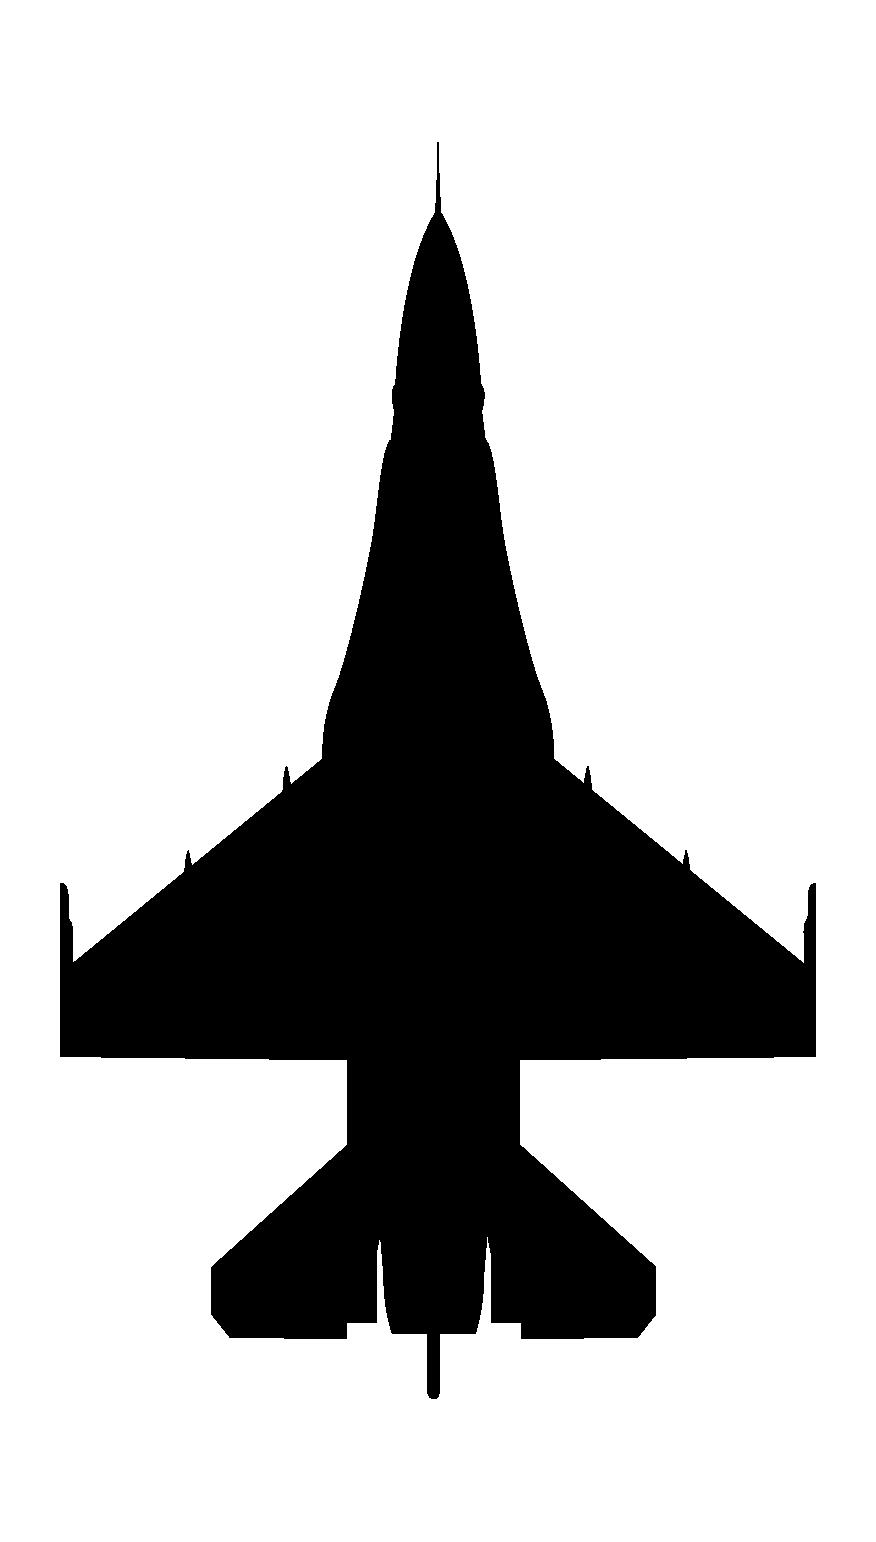
\includegraphics[
                width=7.5mm,
            ]{diagrams/aircraft/silhouette_f16_top.pdf}
        };
        
        \node[yshift=-3mm] (2fig) at (2) {
            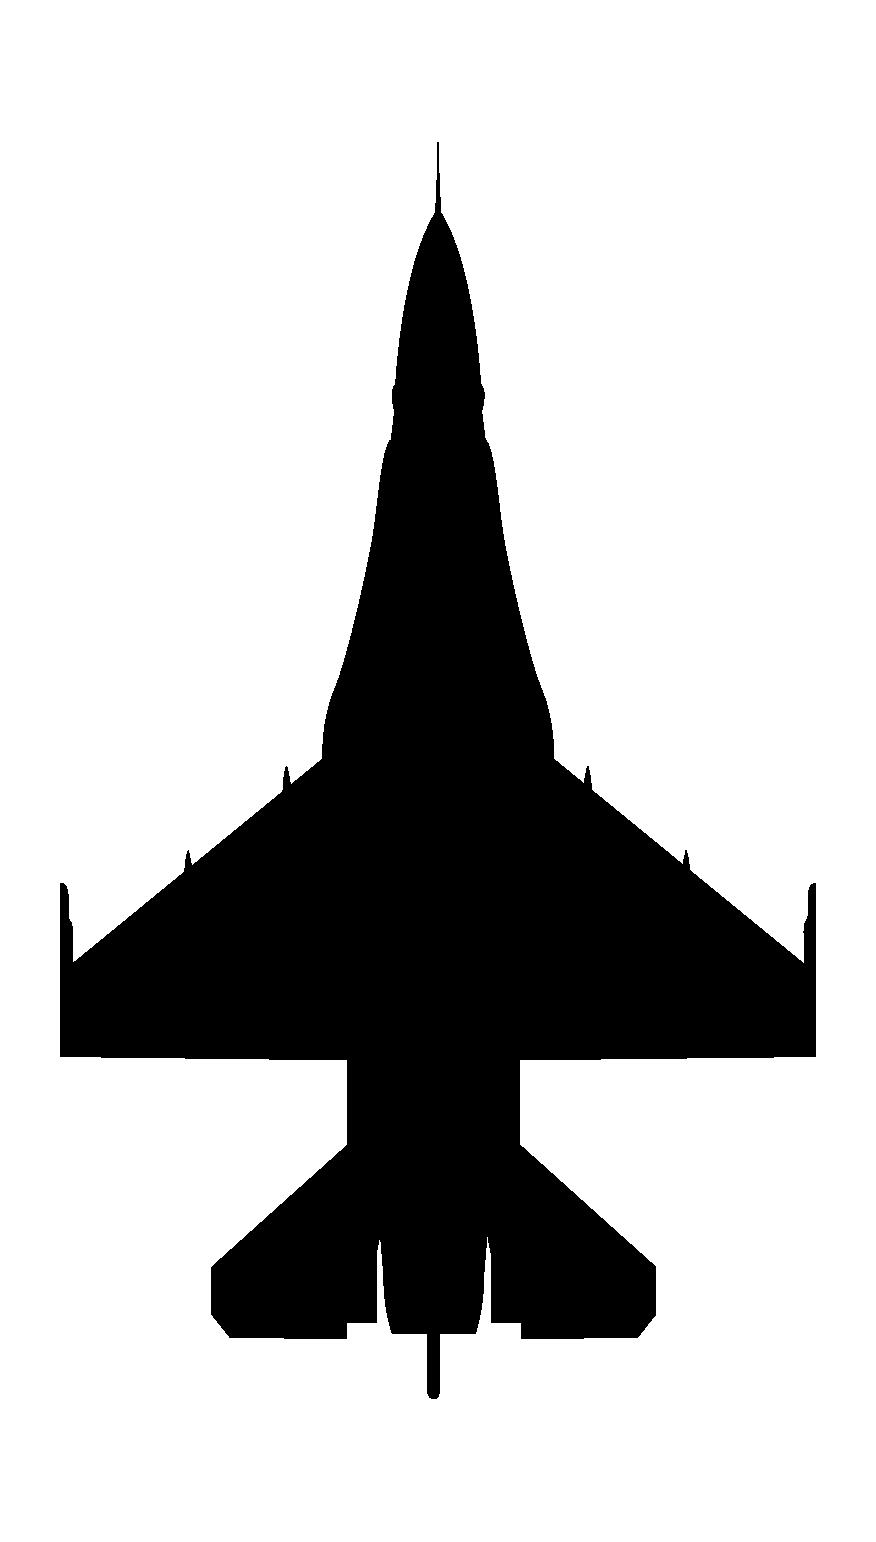
\includegraphics[
                width=7.5mm,
            ]{diagrams/aircraft/silhouette_f16_top.pdf}
        };

        \node[yshift=-3mm] (3fig) at (3) {
            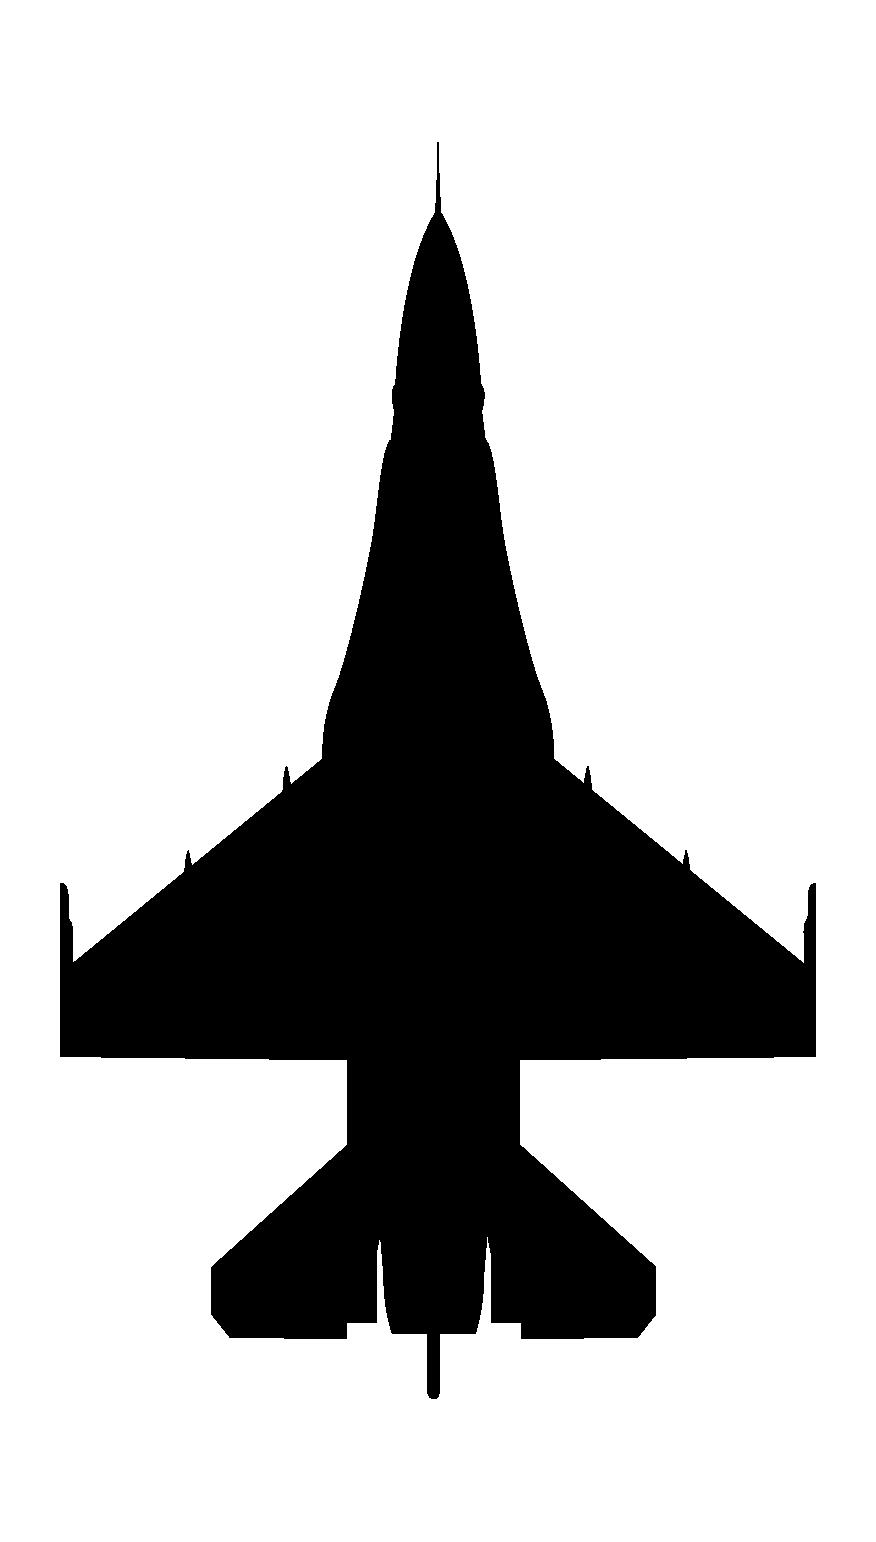
\includegraphics[
                width=7.5mm,
            ]{diagrams/aircraft/silhouette_f16_top.pdf}
        };
        
        \node[yshift=-3mm] (4fig) at (4) {
            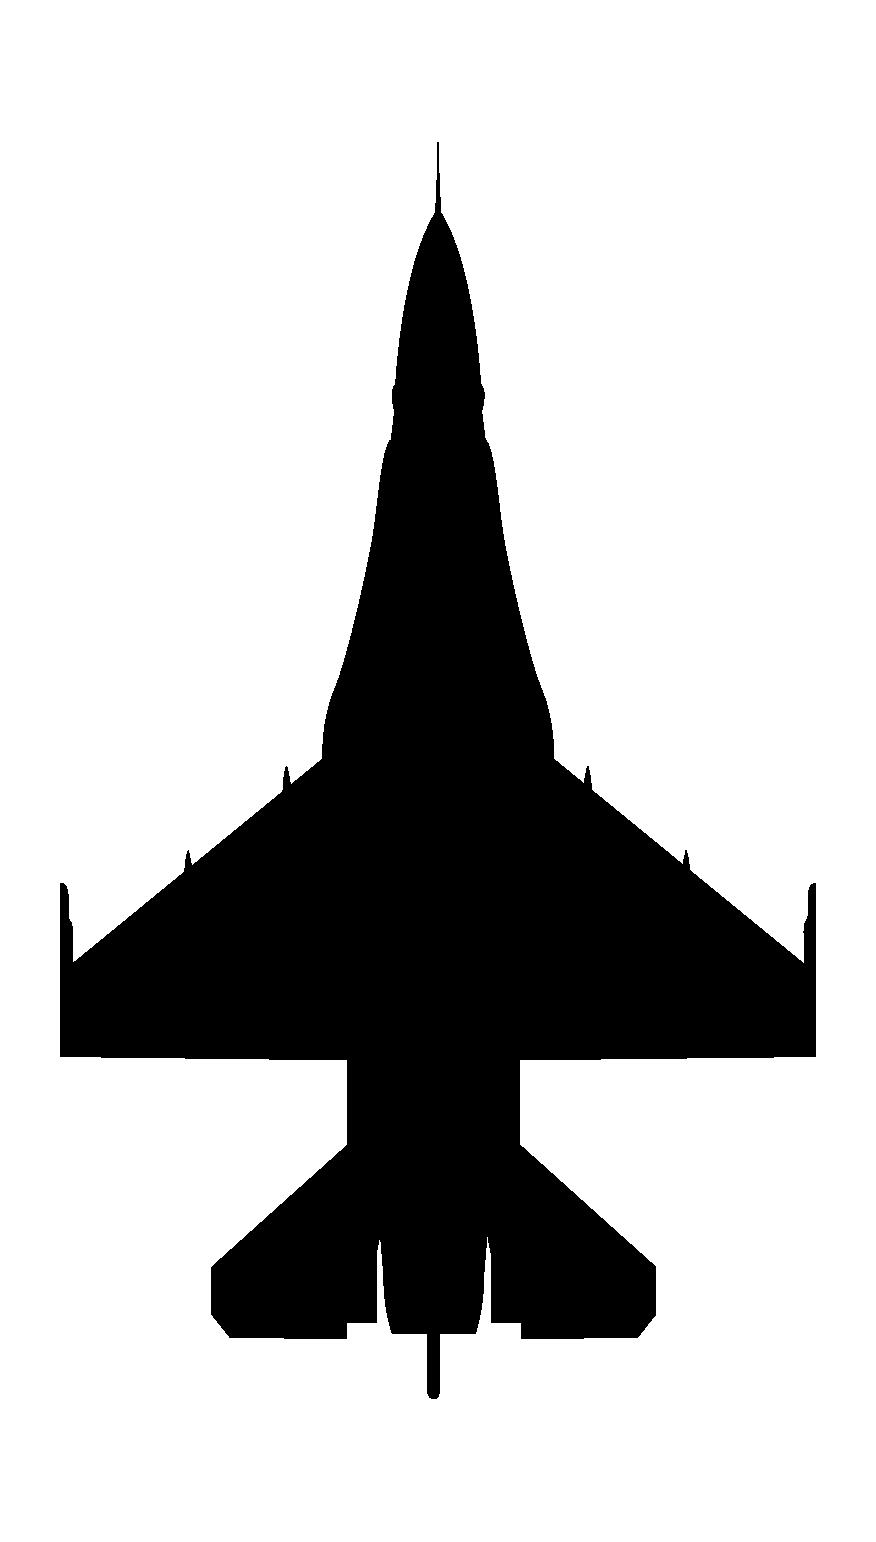
\includegraphics[
                width=7.5mm,
            ]{diagrams/aircraft/silhouette_f16_top.pdf}
        };

        \node[anchor=north, font=\footnotesize] (1label) at (1fig.south) {1};
        \node[anchor=north, font=\footnotesize] (2label) at (2fig.south) {2};
        \node[anchor=north, font=\footnotesize] (3label) at (3fig.south) {3};
        \node[anchor=north, font=\footnotesize] (4label) at (4fig.south) {4};

    \end{tikzpicture}
    \caption{Route}
    \label{fig:supp_fig:form:route}
\end{figure}

\begin{figure}[htbp]
    \centering
    \begin{tikzpicture}[figstyle]
    
        \coordinate (1) at (0,0);
        \coordinate (2) at ($(1)+(190:20)$);
        \coordinate (3) at ($(1)+(0:20)$);
        \coordinate (4) at ($(3)+(-10:20)$);

        % \draw[dashed]
        % (lead) -- ++(0:20) arc (0:-20:20) -- (lead);

        \draw[fill=color2!15]
        ($(1)+(180:10)$) 
        -- ++(180:20) 
        node[font=\footnotesize, above, pos=0.5] {0.6-1.0 nm}
        node[font=\footnotesize, left, pos=1] {0$^\circ$}
        arc (180:210:30)
        node[font=\footnotesize, left, pos=1] {30$^\circ$}
        -- ($(1)+(210:10)$) 
        arc (210:180:10);
        \draw[]
        (1) -- (3)
        node[font=\footnotesize, above, pos=0.5] {LAB};
        \draw[fill=color2!15]
        ($(3)+(0:10)$) 
        -- ++(0:20) node[font=\footnotesize, above, pos=0.5] {0.6-1.0 nm}
        node[font=\footnotesize, right, pos=1] {0$^\circ$}
        arc (0:-30:30)
        node[font=\footnotesize, right, pos=1] {30$^\circ$}
        -- ($(3)+(-30:10)$) 
        arc (-30:0:10);

        \node[yshift=-3mm] (1fig) at (1) {
            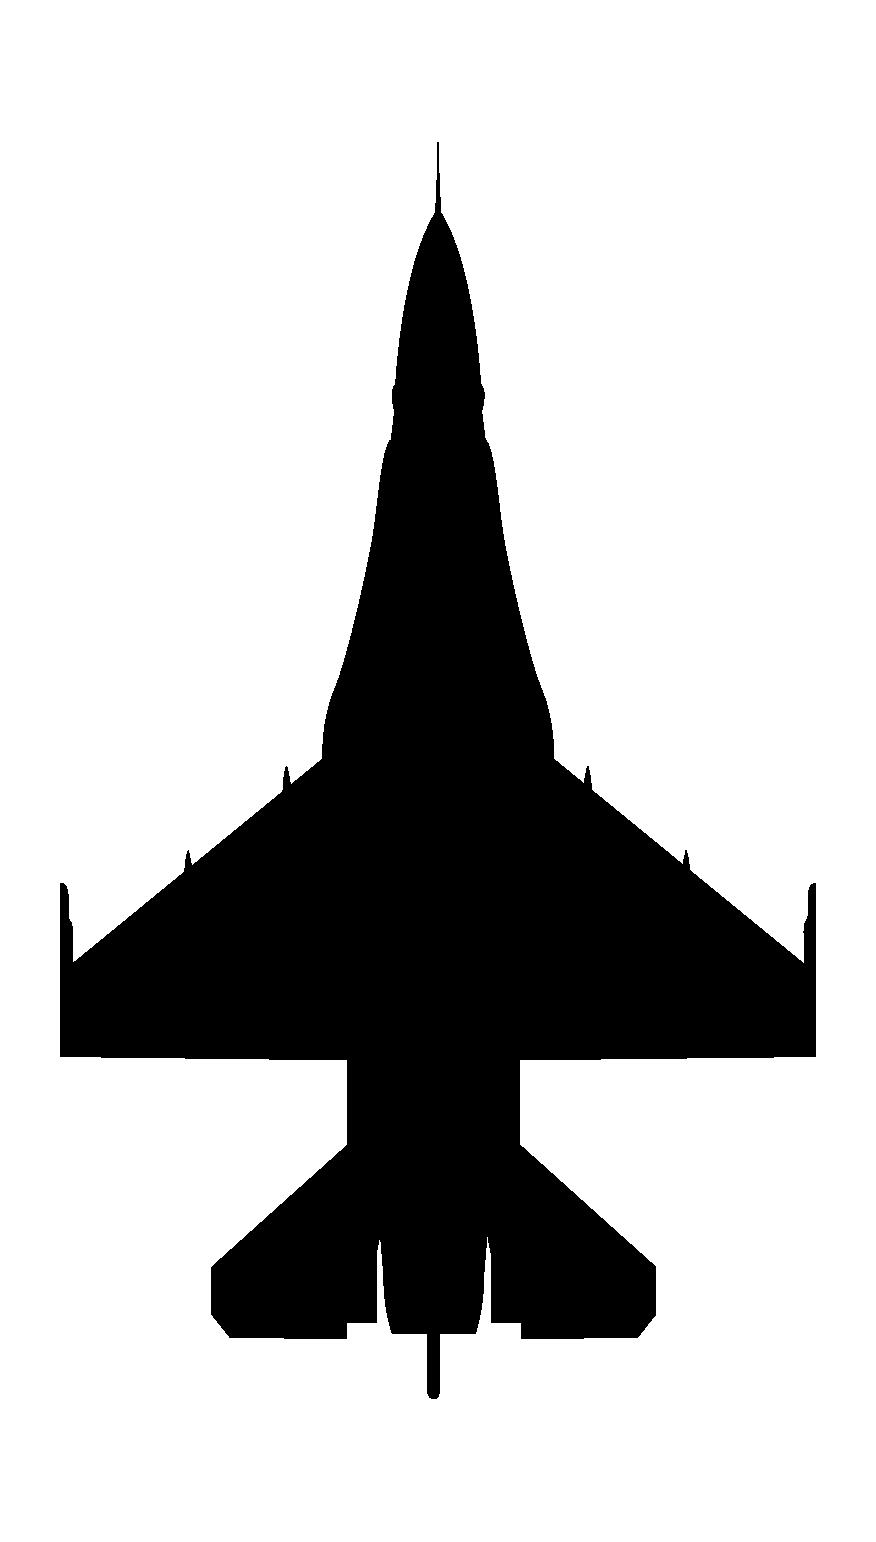
\includegraphics[
                width=7.5mm,
            ]{diagrams/aircraft/silhouette_f16_top.pdf}
        };
        
        \node[yshift=-3mm] (2fig) at (2) {
            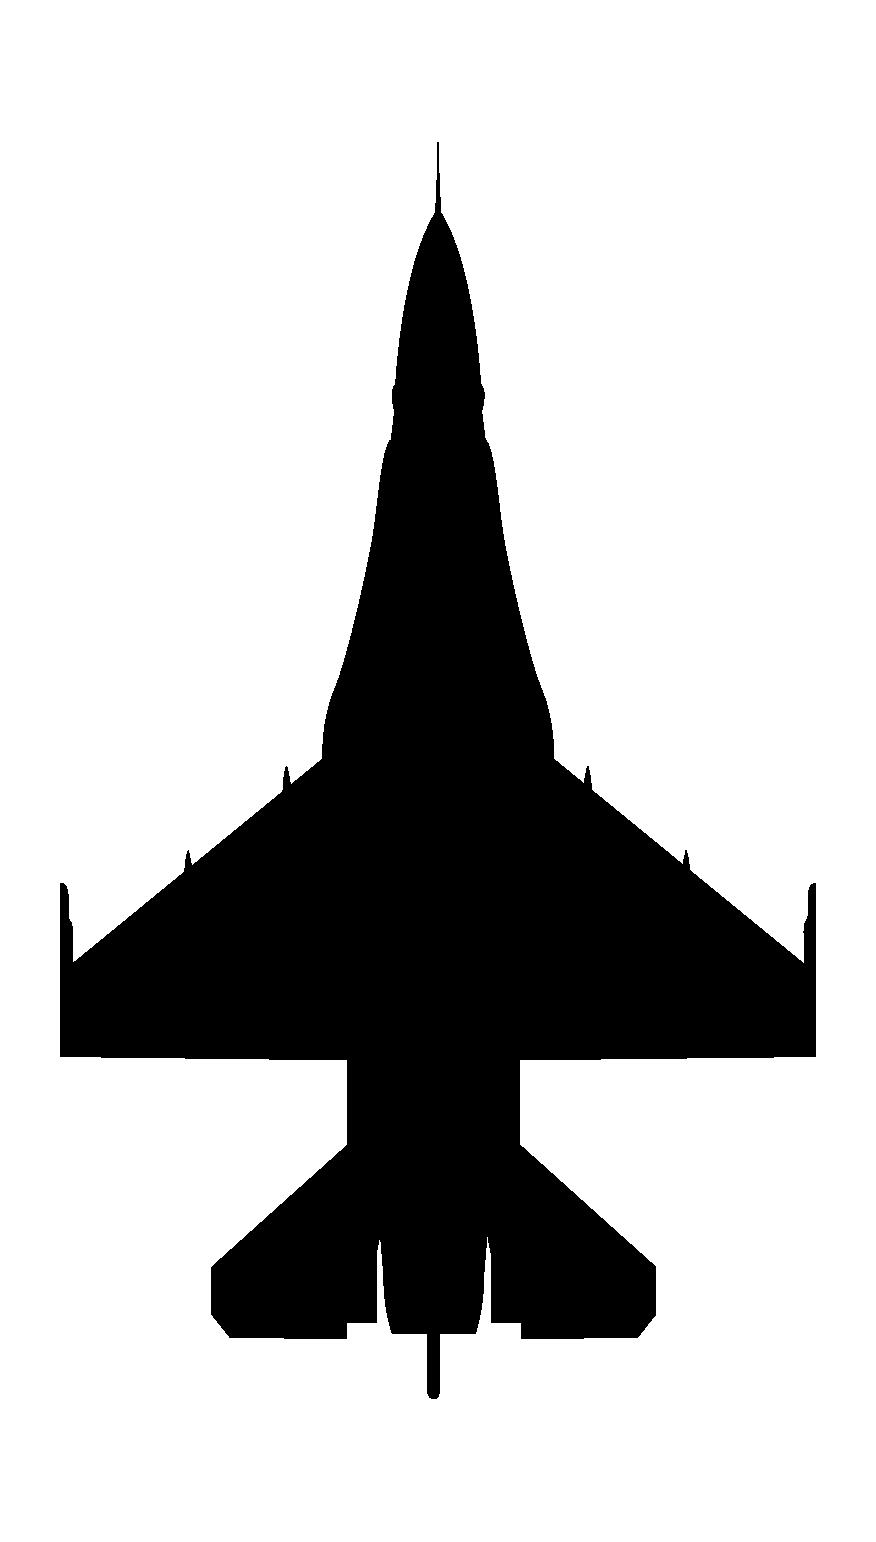
\includegraphics[
                width=7.5mm,
            ]{diagrams/aircraft/silhouette_f16_top.pdf}
        };

        \node[yshift=-3mm] (3fig) at (3) {
            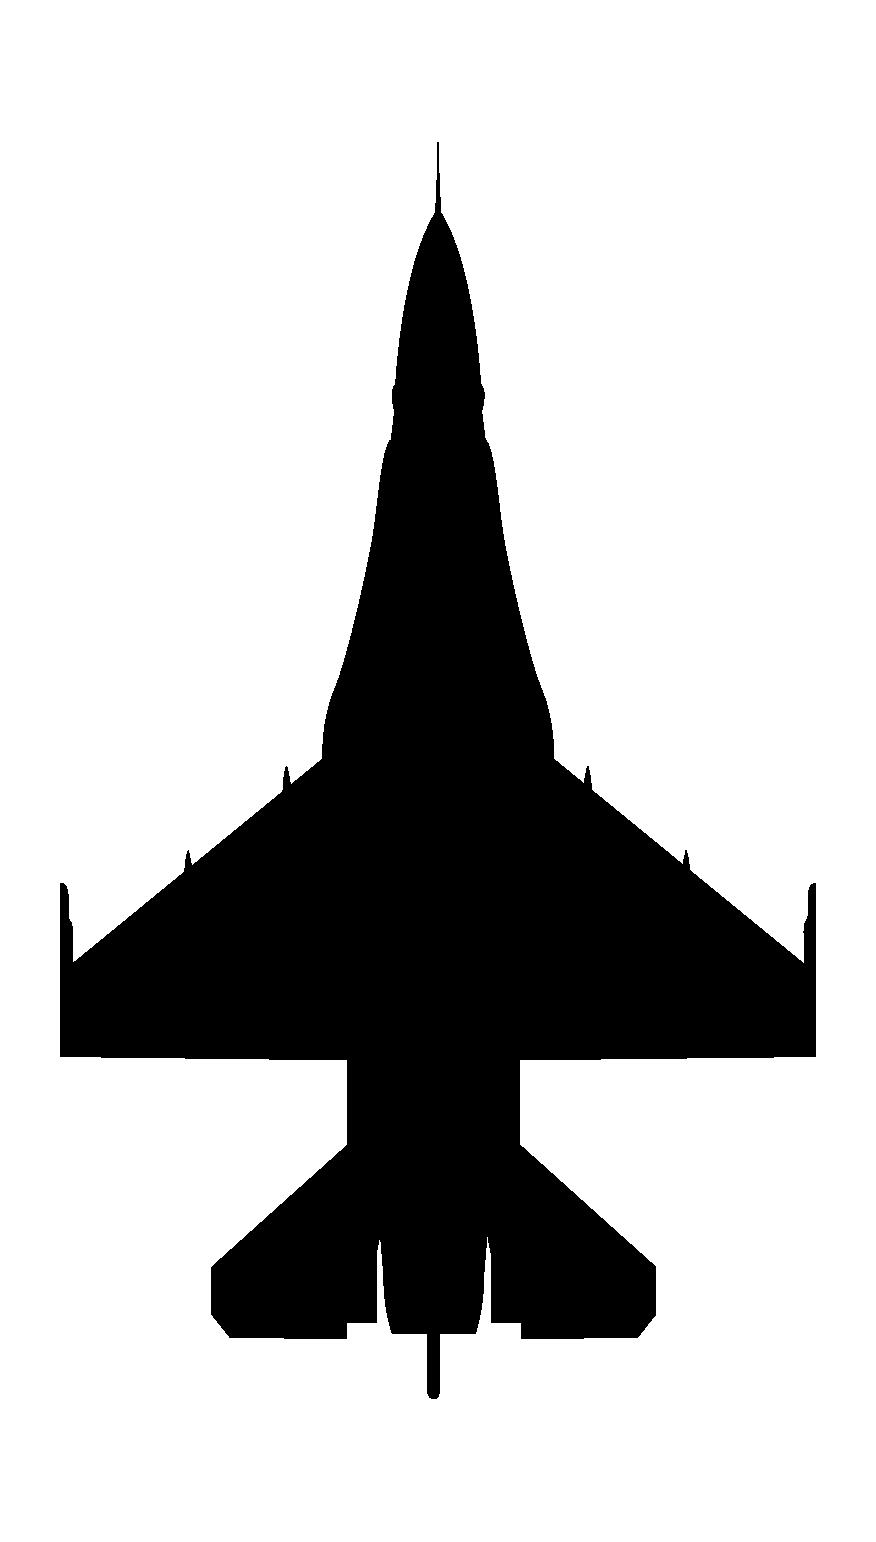
\includegraphics[
                width=7.5mm,
            ]{diagrams/aircraft/silhouette_f16_top.pdf}
        };
        
        \node[yshift=-3mm] (4fig) at (4) {
            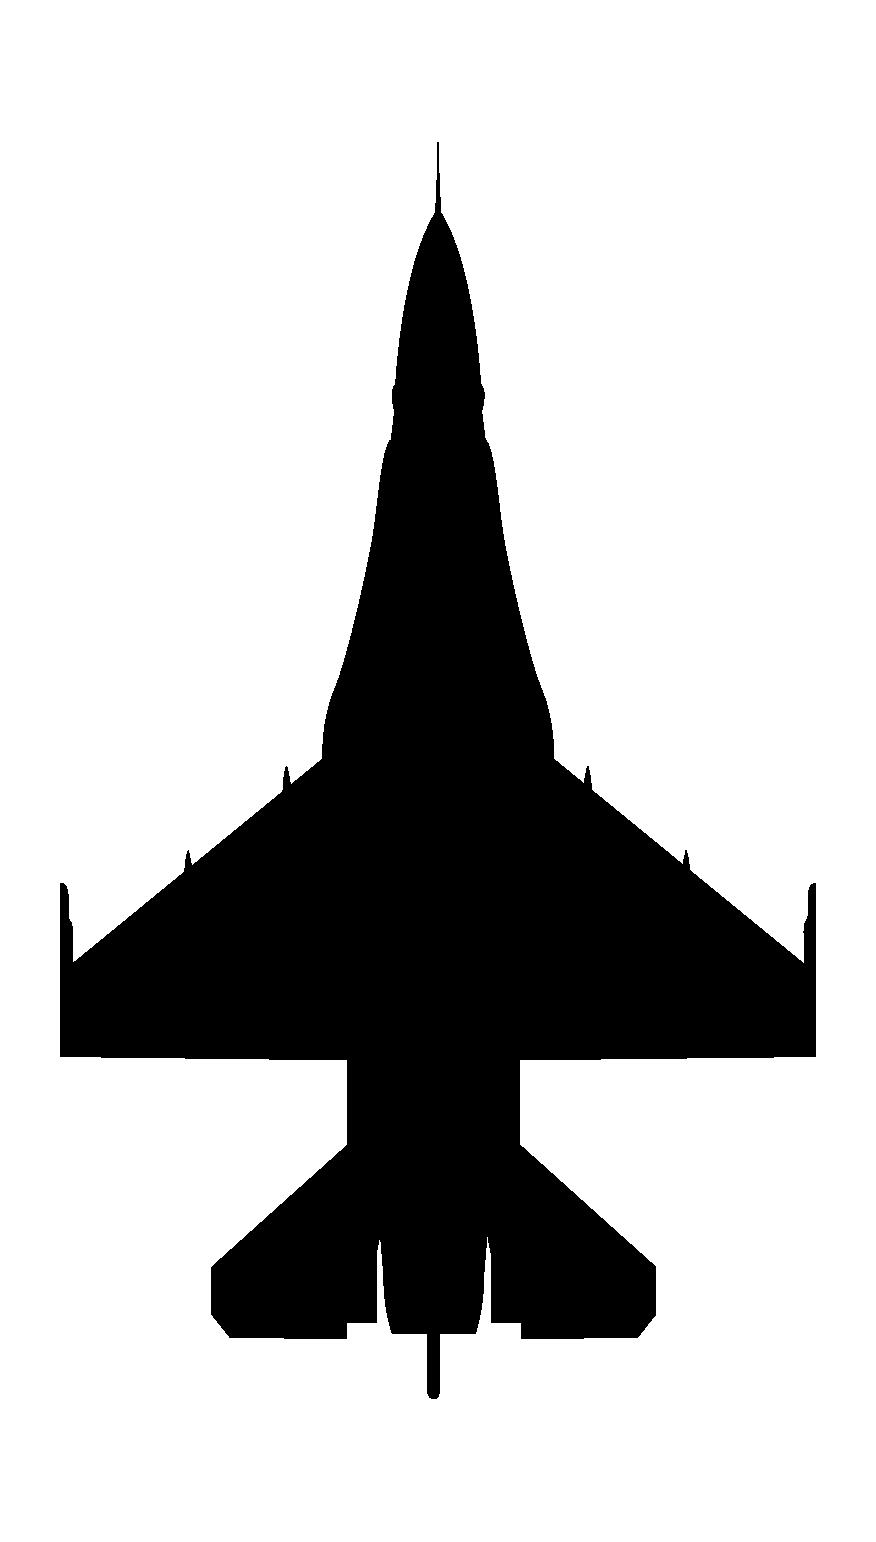
\includegraphics[
                width=7.5mm,
            ]{diagrams/aircraft/silhouette_f16_top.pdf}
        };

        \node[anchor=north, font=\footnotesize] (1label) at (1fig.south) {1};
        \node[anchor=north, font=\footnotesize] (2label) at (2fig.south) {2};
        \node[anchor=north, font=\footnotesize] (3label) at (3fig.south) {3};
        \node[anchor=north, font=\footnotesize] (4label) at (4fig.south) {4};

    \end{tikzpicture}
    \caption{Spread}
    \label{fig:supp_fig:form:spread}
\end{figure}

\begin{figure}[htbp]
    \centering
    \begin{tikzpicture}[figstyle]
    
        \coordinate (1) at (0,0);
        \coordinate (2) at ($(1)+(220:20)$);
        \coordinate (3) at ($(1)+(0:20)$);
        \coordinate (4) at ($(3)+(-40:20)$);

        % \draw[dashed]
        % (lead) -- ++(0:20) arc (0:-20:20) -- (lead);

        \draw[fill=color2!15]
        ($(1)+(210:10)$) 
        -- ++(210:20) 
        node[font=\footnotesize, above left, pos=0.5] {Fighting Wing}
        node[font=\footnotesize, left, pos=1] {30$^\circ$}
        arc (210:240:30)
        node[font=\footnotesize, below, pos=1] {60$^\circ$}
        -- ($(1)+(240:10)$) 
        node[font=\footnotesize, right, pos=0.25] {2}
        arc (240:210:10);
        \draw[]
        (1) -- (3)
        node[font=\footnotesize, above, pos=0.5] {LAB};
        \draw[fill=color2!15]
        ($(3)+(-30:10)$) 
        -- ++(-30:20) 
        node[font=\footnotesize, above right, pos=0.5] {Fighting Wing}
        node[font=\footnotesize, right, pos=1] {30$^\circ$}
        arc (-30:-60:30)
        node[font=\footnotesize, below, pos=1] {60$^\circ$}
        -- ($(3)+(-60:10)$) 
        node[font=\footnotesize, left, pos=0.25] {4}
        arc (-60:-30:10);

        \node[yshift=-3mm] (1fig) at (1) {
            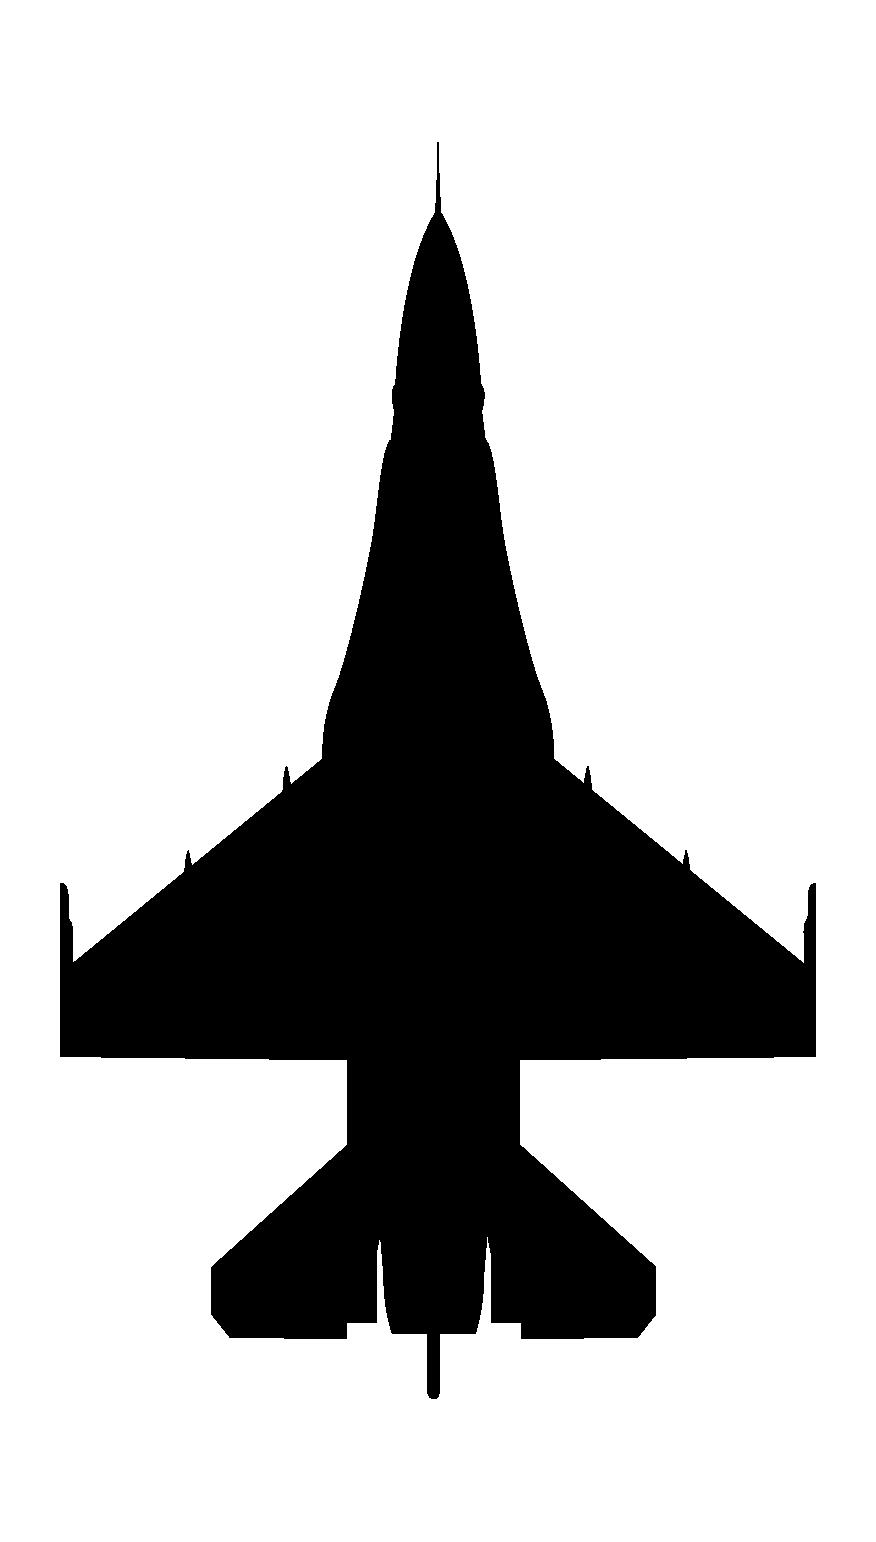
\includegraphics[
                width=7.5mm,
            ]{diagrams/aircraft/silhouette_f16_top.pdf}
        };
        
        \node[yshift=-3mm] (2fig) at (2) {
            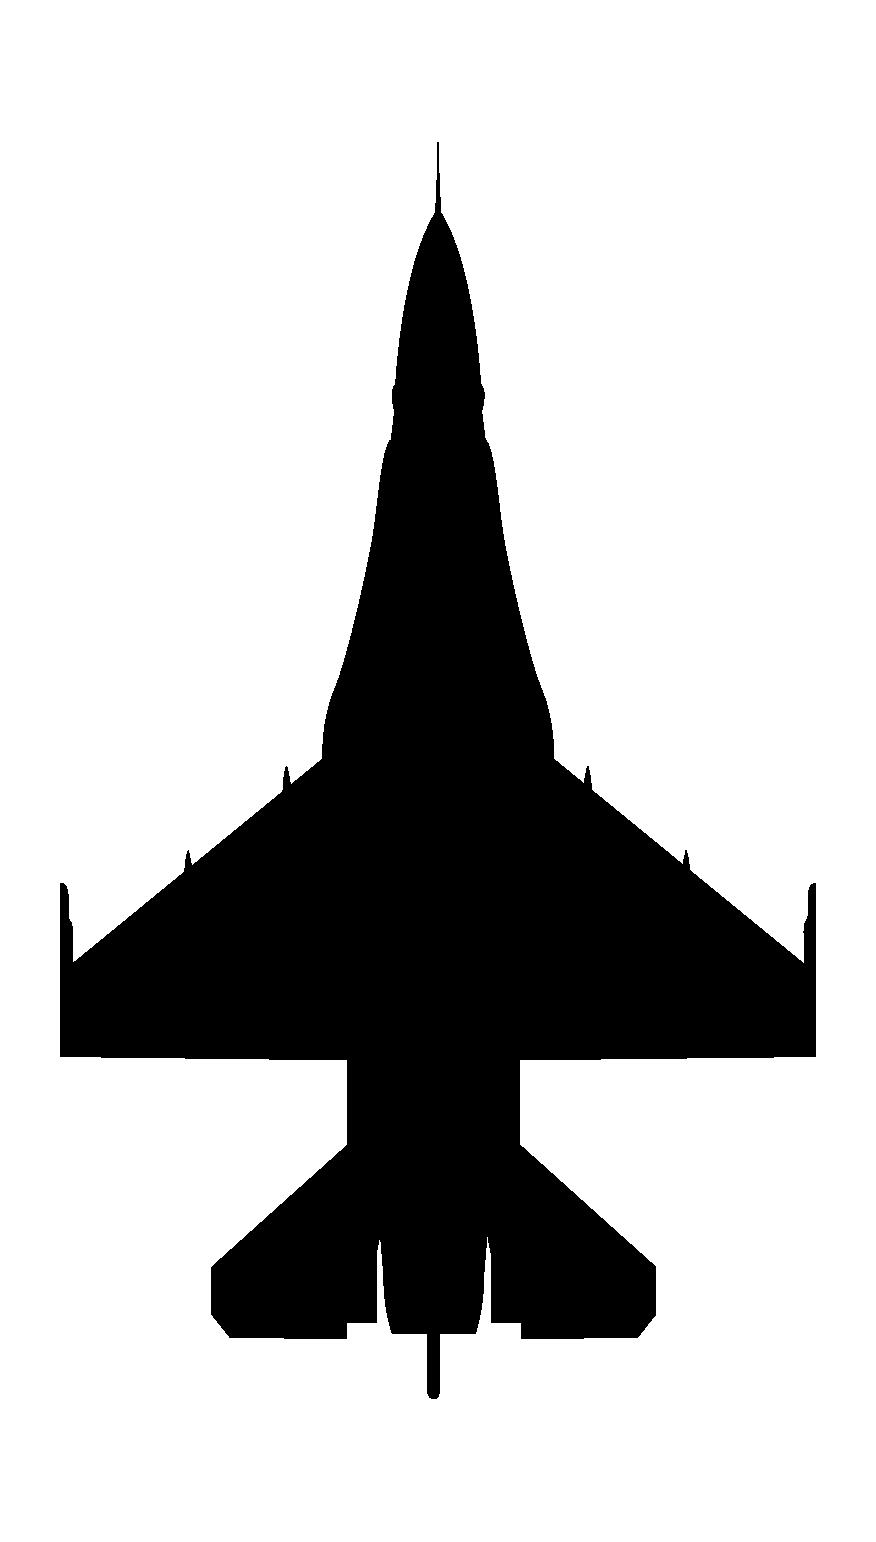
\includegraphics[
                width=7.5mm,
            ]{diagrams/aircraft/silhouette_f16_top.pdf}
        };

        \node[yshift=-3mm] (3fig) at (3) {
            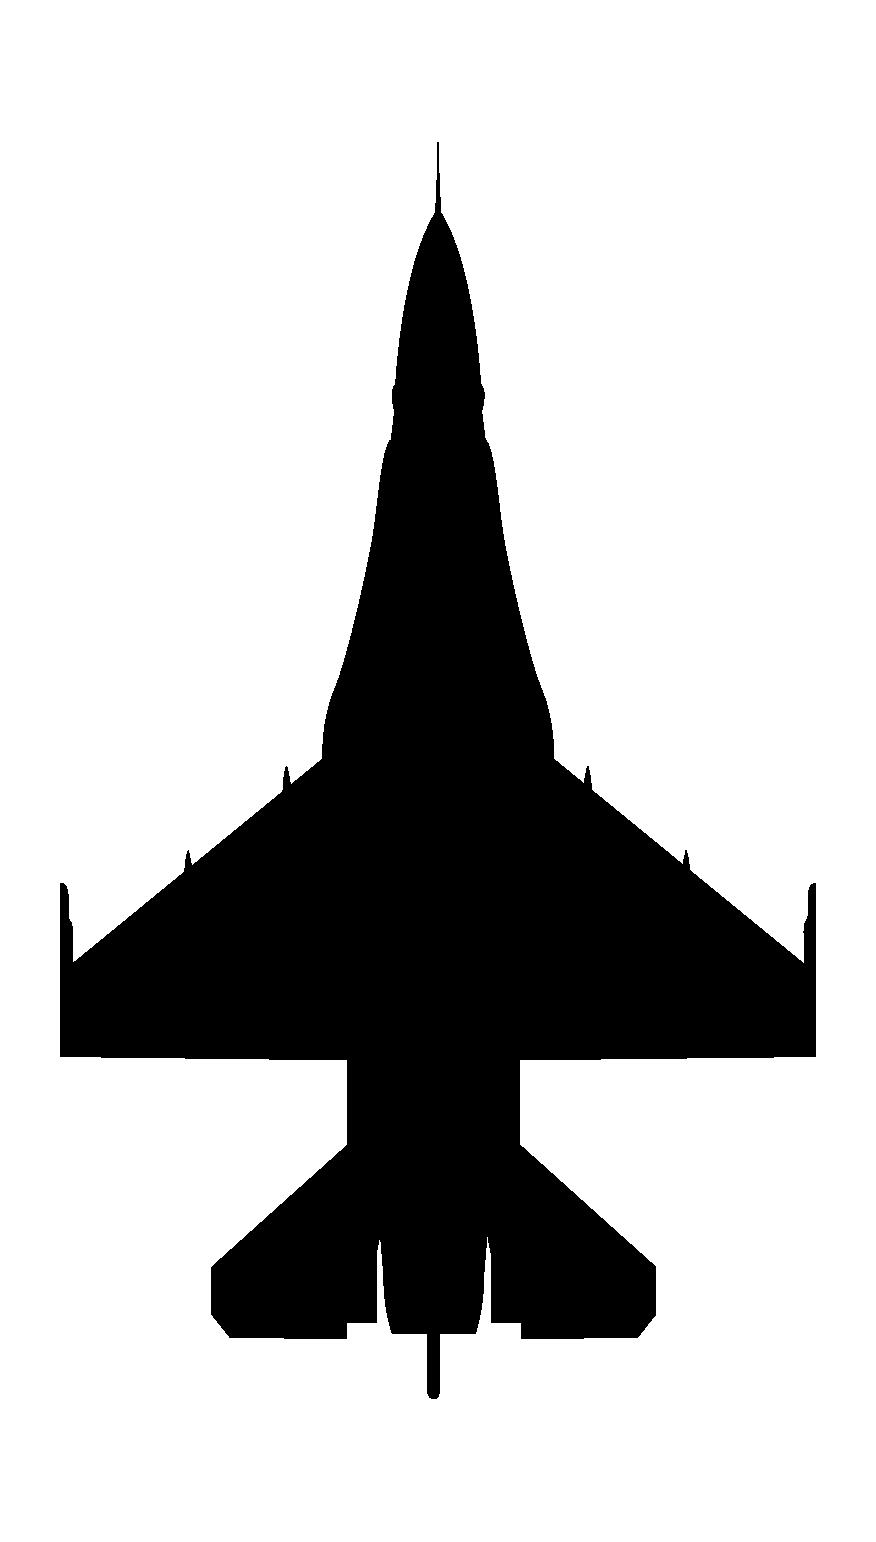
\includegraphics[
                width=7.5mm,
            ]{diagrams/aircraft/silhouette_f16_top.pdf}
        };
        
        \node[yshift=-3mm] (4fig) at (4) {
            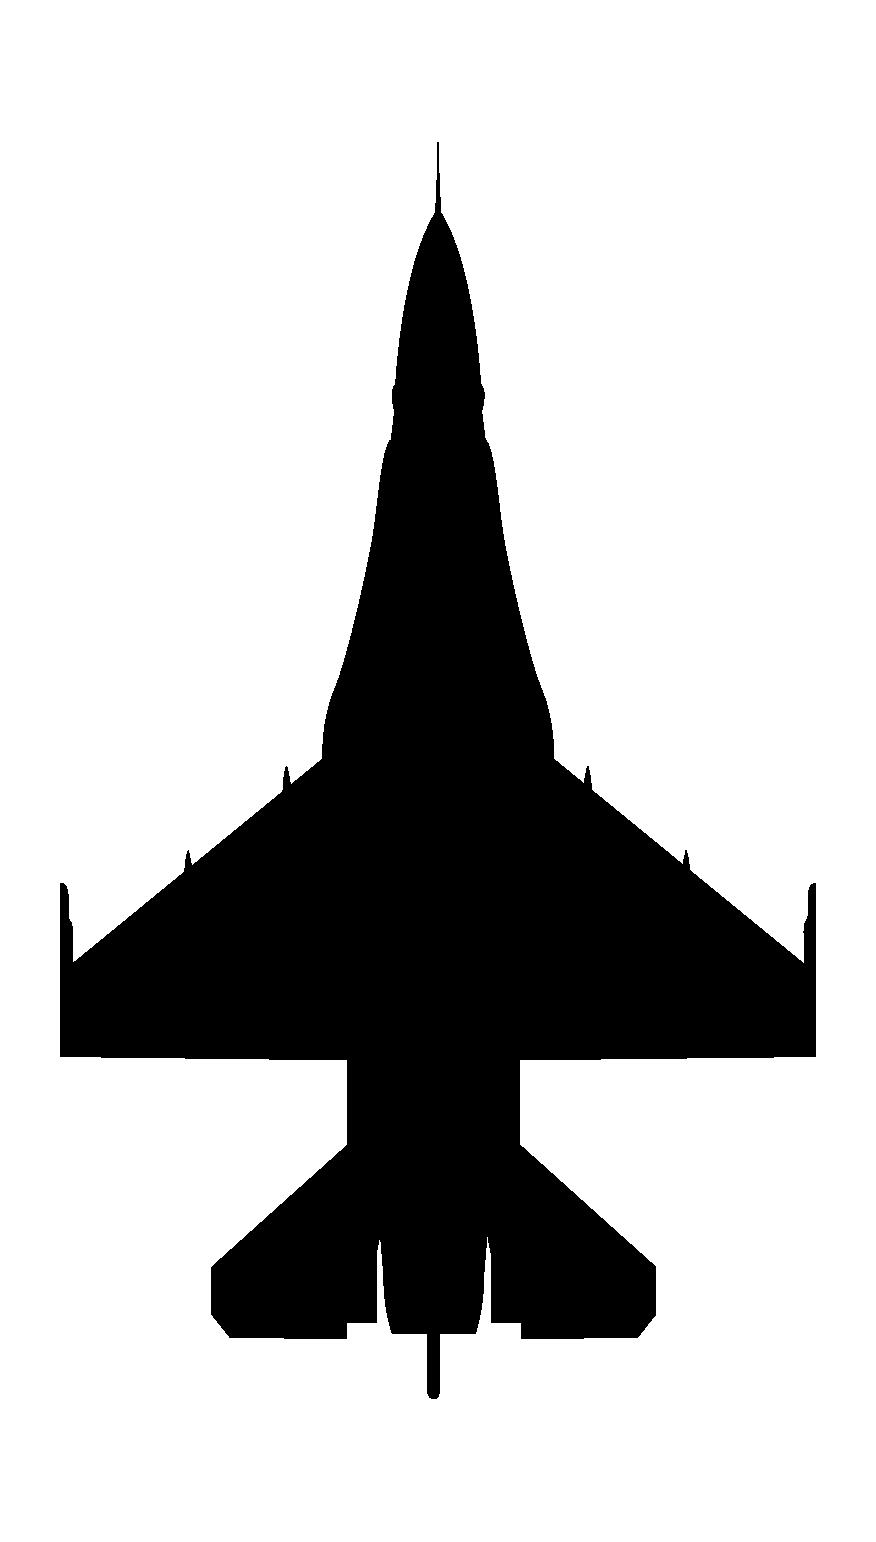
\includegraphics[
                width=7.5mm,
            ]{diagrams/aircraft/silhouette_f16_top.pdf}
        };

        \node[anchor=north, font=\footnotesize] (1label) at (1fig.south) {1};
        \node[anchor=north, font=\footnotesize] (3label) at (3fig.south) {3};

    \end{tikzpicture}
    \caption{Fluid Four}
    \label{fig:supp_fig:form:fluidfour}
\end{figure}

\begin{figure}[htbp]
    \centering
    \begin{tikzpicture}[figstyle]
    
        \coordinate (1) at (0,0);
        \coordinate (2) at ($(1)+(210:10)$);
        \coordinate (3) at ($(1)+(0:20)$);
        \coordinate (4) at ($(3)+(-30:10)$);

        \draw[]
        (1) -- (2);
        \draw[]
        (1) -- (3)
        node[font=\footnotesize, above, pos=0.5] {LAB};
        \draw[]
        (3) -- (4);

        \node[yshift=-3mm] (1fig) at (1) {
            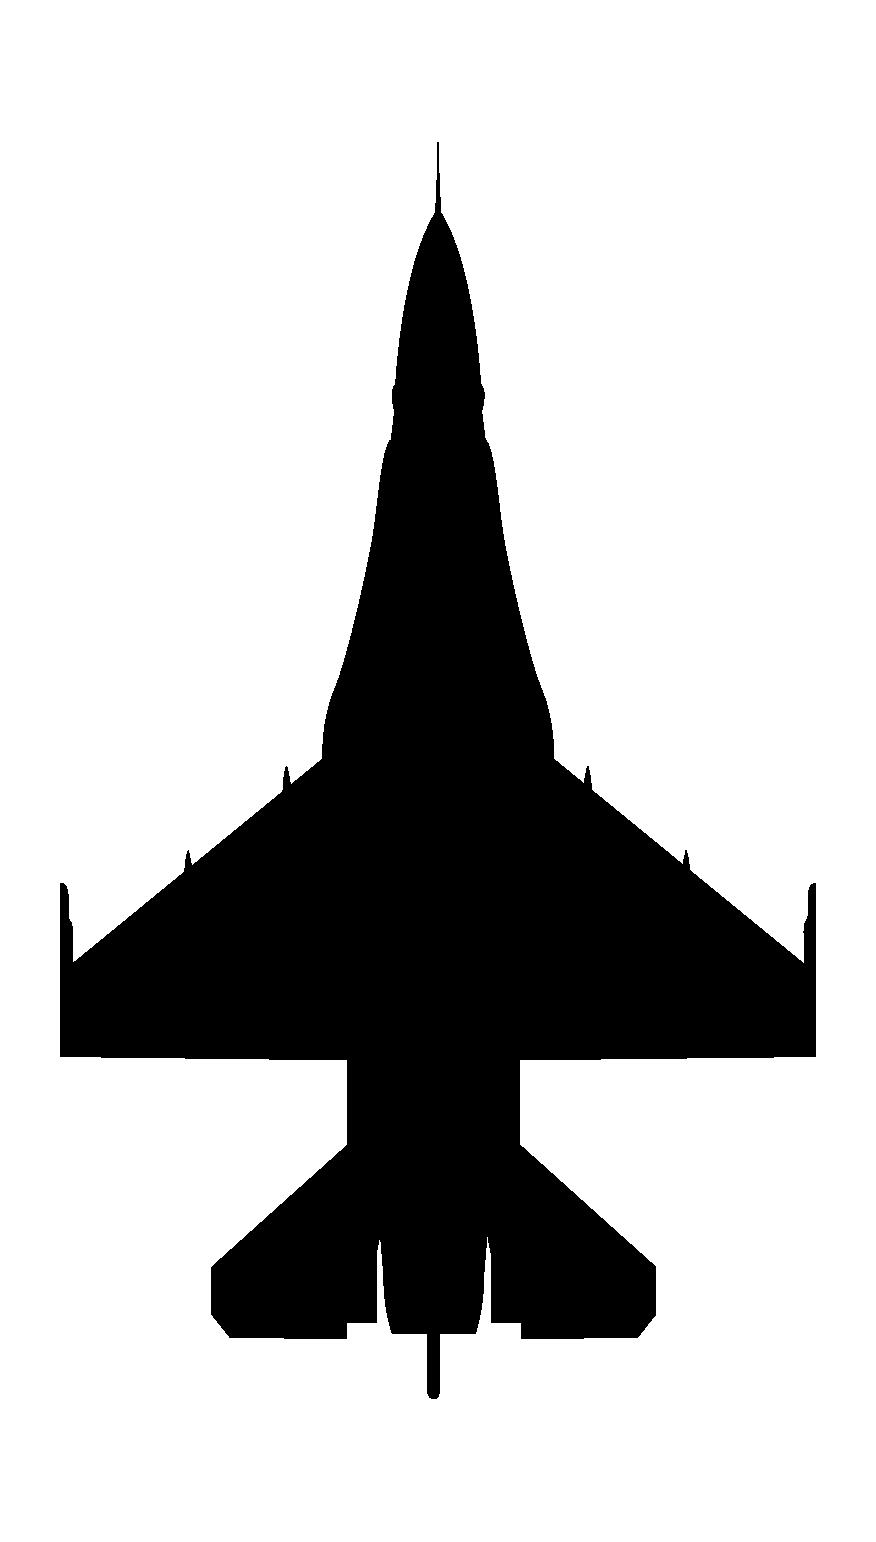
\includegraphics[
                width=7.5mm,
            ]{diagrams/aircraft/silhouette_f16_top.pdf}
        };
        
        \node[yshift=-3mm] (2fig) at (2) {
            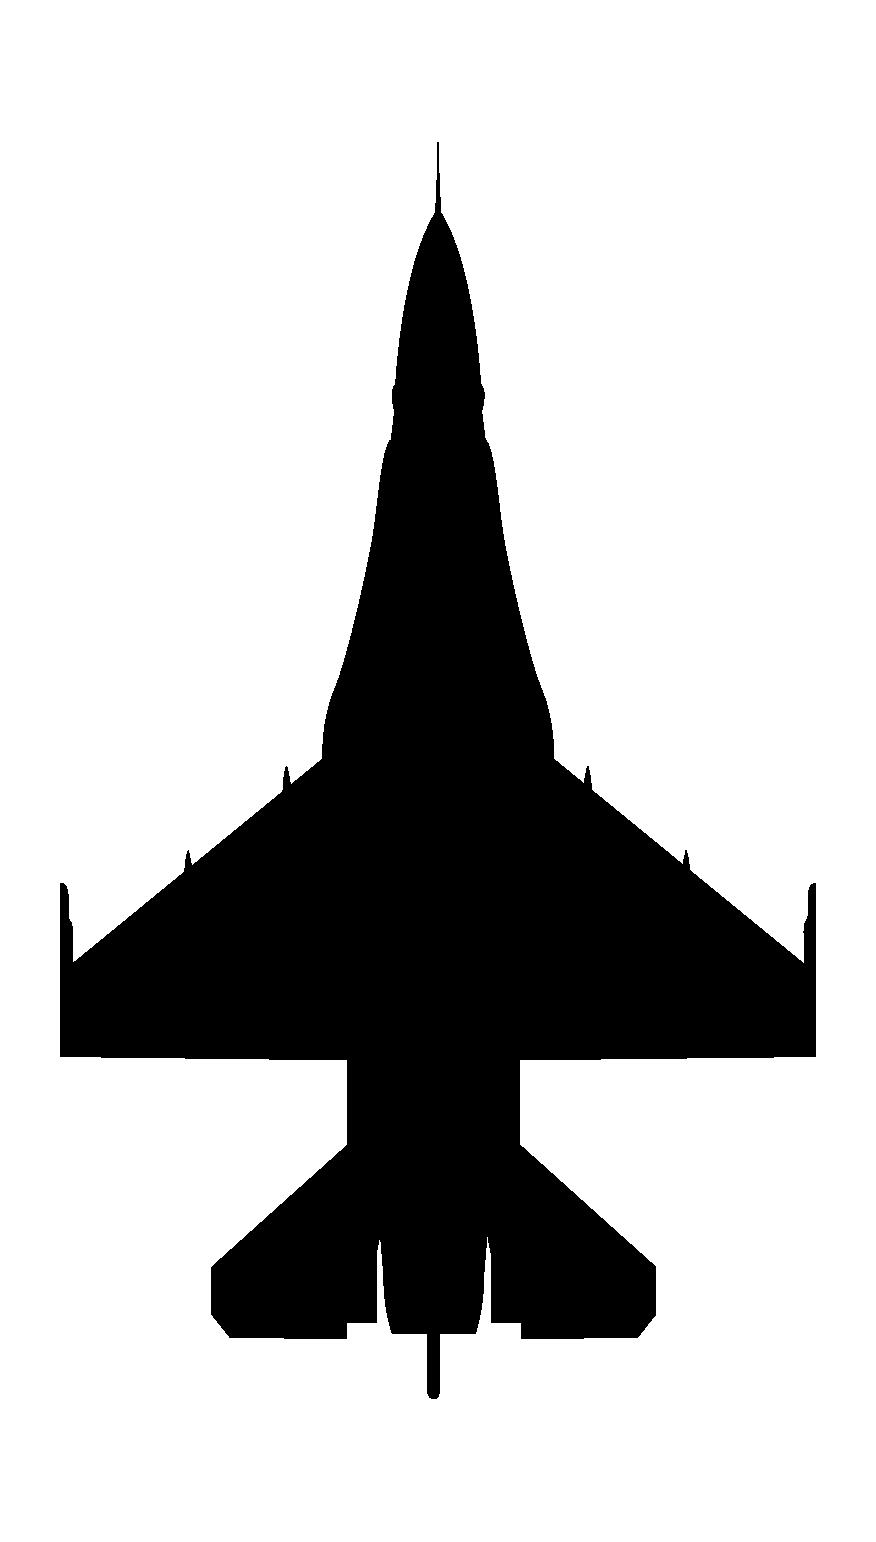
\includegraphics[
                width=7.5mm,
            ]{diagrams/aircraft/silhouette_f16_top.pdf}
        };

        \node[yshift=-3mm] (3fig) at (3) {
            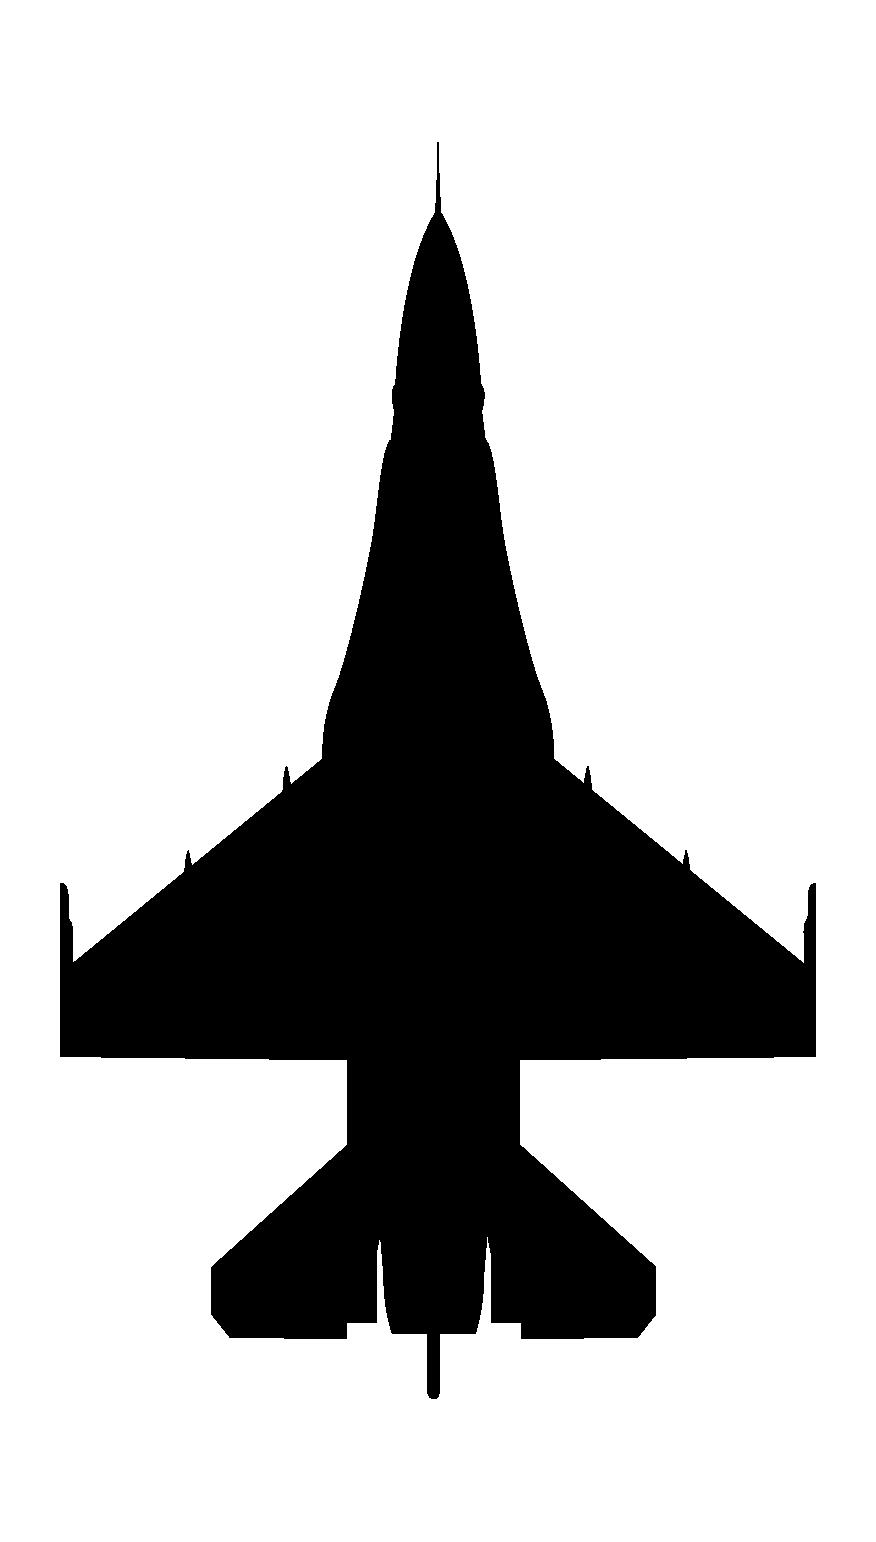
\includegraphics[
                width=7.5mm,
            ]{diagrams/aircraft/silhouette_f16_top.pdf}
        };
        
        \node[yshift=-3mm] (4fig) at (4) {
            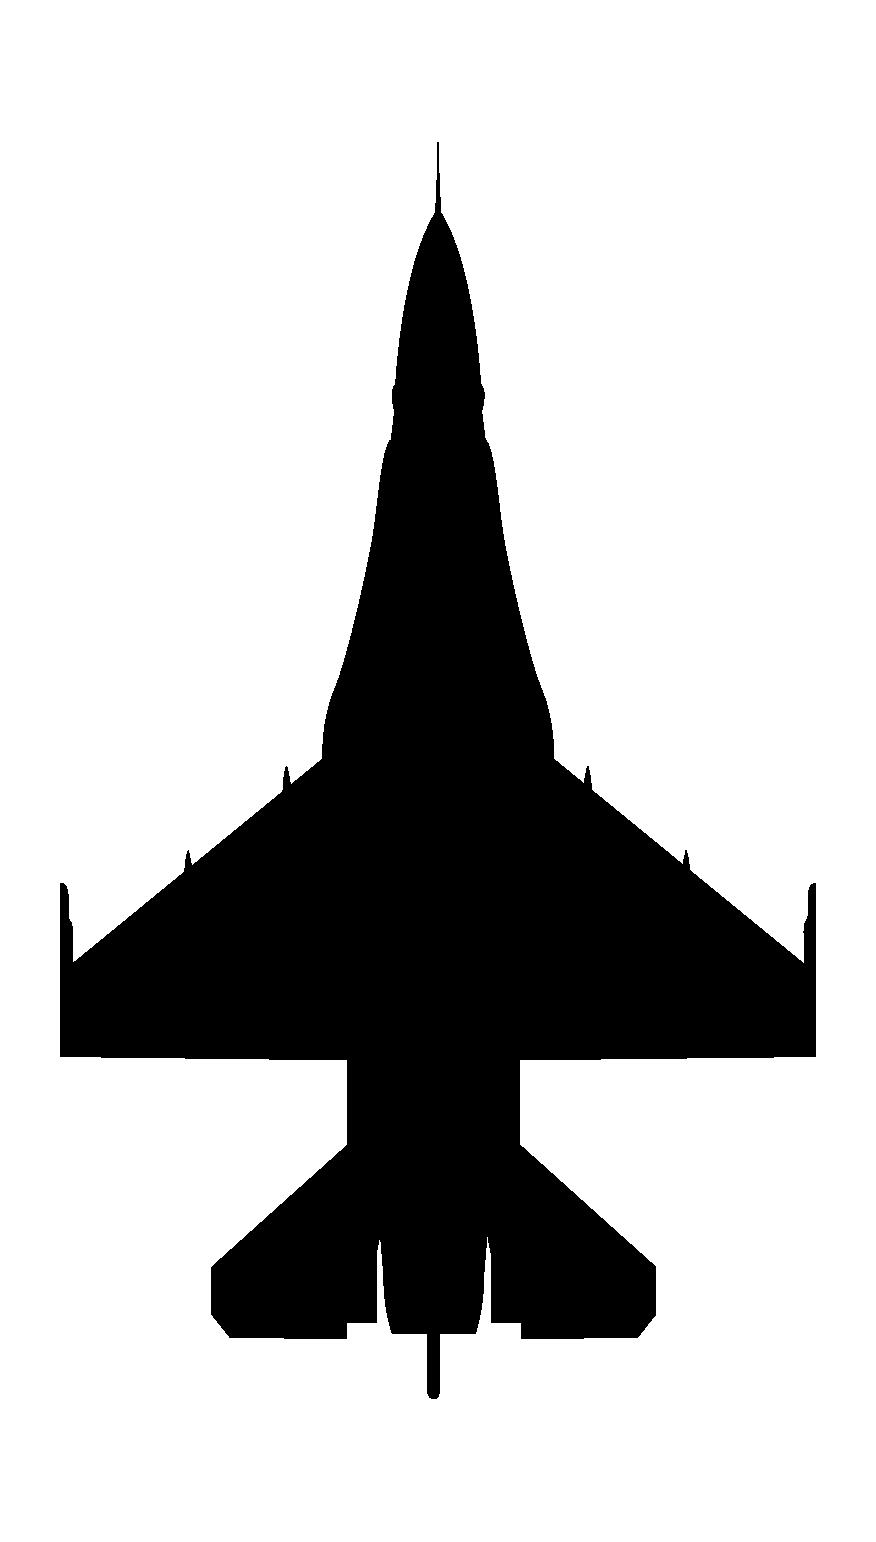
\includegraphics[
                width=7.5mm,
            ]{diagrams/aircraft/silhouette_f16_top.pdf}
        };

        \node[anchor=north, font=\footnotesize] (1label) at (1fig.south) {1};
        \node[anchor=north, font=\footnotesize] (2label) at (2fig.south) {2};
        \node[anchor=north, font=\footnotesize] (3label) at (3fig.south) {3};
        \node[anchor=north, font=\footnotesize] (4label) at (4fig.south) {4};

        \node[anchor=east, font=\footnotesize] at (2fig.west) {Fingertip};
        \node[anchor=west, font=\footnotesize] at (4fig.east) {Fingertip};

    \end{tikzpicture}
    \caption{Res Cell}
    \label{fig:supp_fig:form:rescell}
\end{figure}

\begin{figure}[htbp]
    \centering
    \begin{tikzpicture}[figstyle]
        
        \coordinate (1) at (0,0);
        \coordinate (2) at ($(1)+(20,0)$);
        \coordinate (3) at ($(1)+(10,-30)$);
        \coordinate (4) at ($(3)+(20,0)$);

        \draw[<->]
        ($(1)+(-5,0)$) 
        -- ($(3)+(-15,0)$)
        node[font=\footnotesize, pos=0.5, rotate=90, above] {1.5-3.0 nm};
        \draw[thin]
        (1) -- ($(1)+(-7,0)$)
        (3) -- ($(3)+(-17,0)$);

        \draw[<->]
        ($(1)+(0,5)$) 
        -- ($(2)+(0,5)$)
        node[font=\footnotesize, pos=0.5, above] {LAB};
        \draw[thin]
        (1) -- ($(1)+(0,7)$)
        (2) -- ($(2)+(0,7)$);

        \draw[<->]
        ($(3)+(0,5)$) 
        -- ($(4)+(0,5)$)
        node[font=\footnotesize, pos=0.5, above] {LAB};
        \draw[thin]
        (3) -- ($(3)+(0,7)$)
        (4) -- ($(4)+(0,7)$);


        \node[yshift=-2mm] (1fig) at (1) {
            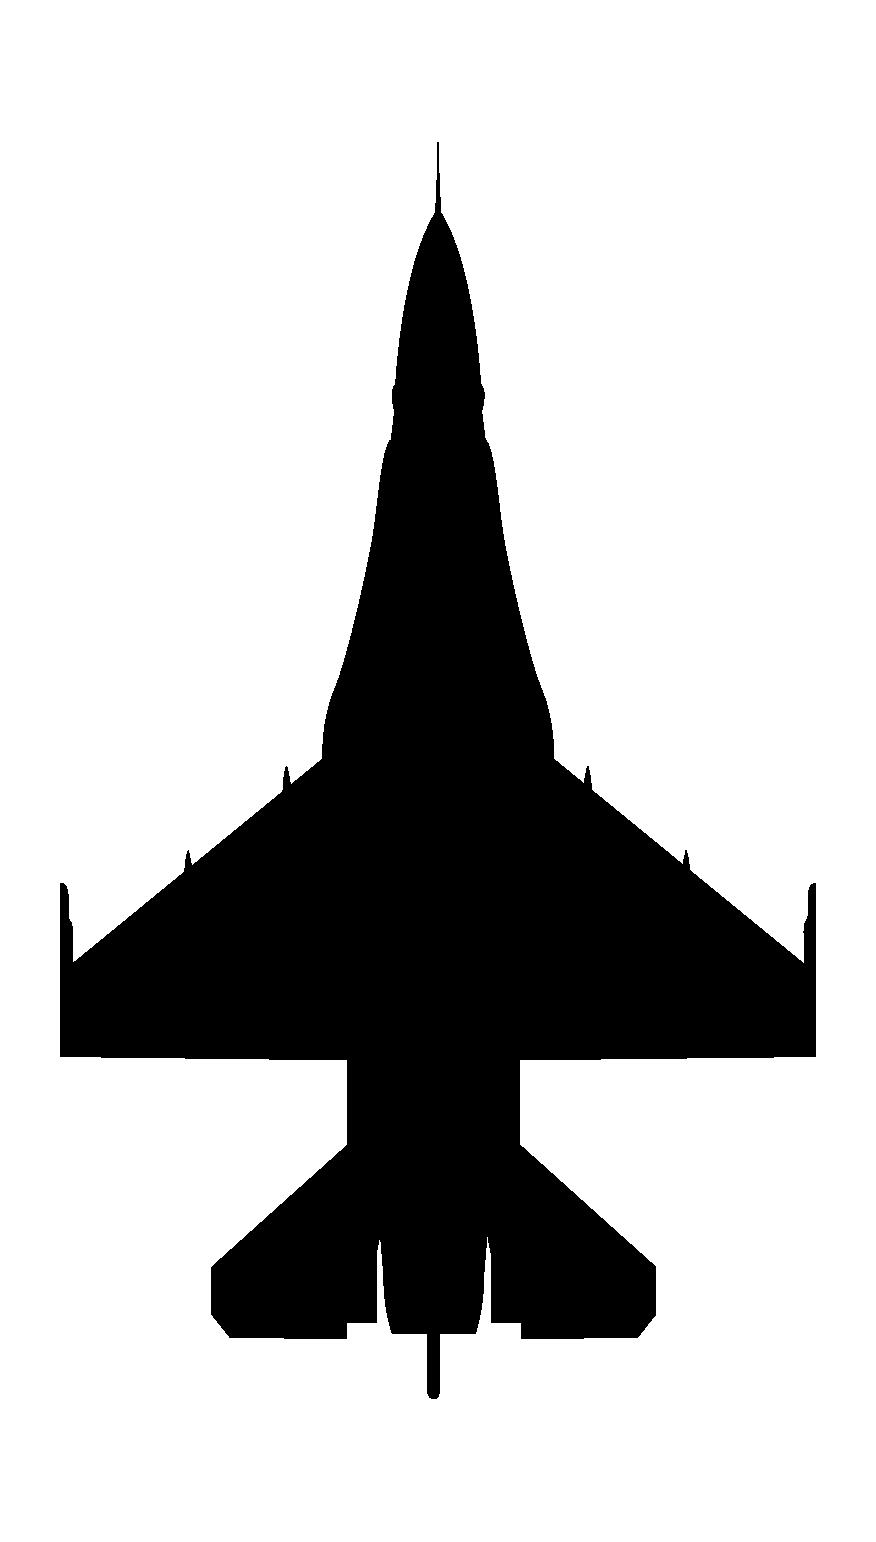
\includegraphics[
                width=7.5mm,
            ]{diagrams/aircraft/silhouette_f16_top.pdf}
        };
        
        \node[yshift=-2mm] (2fig) at (2) {
            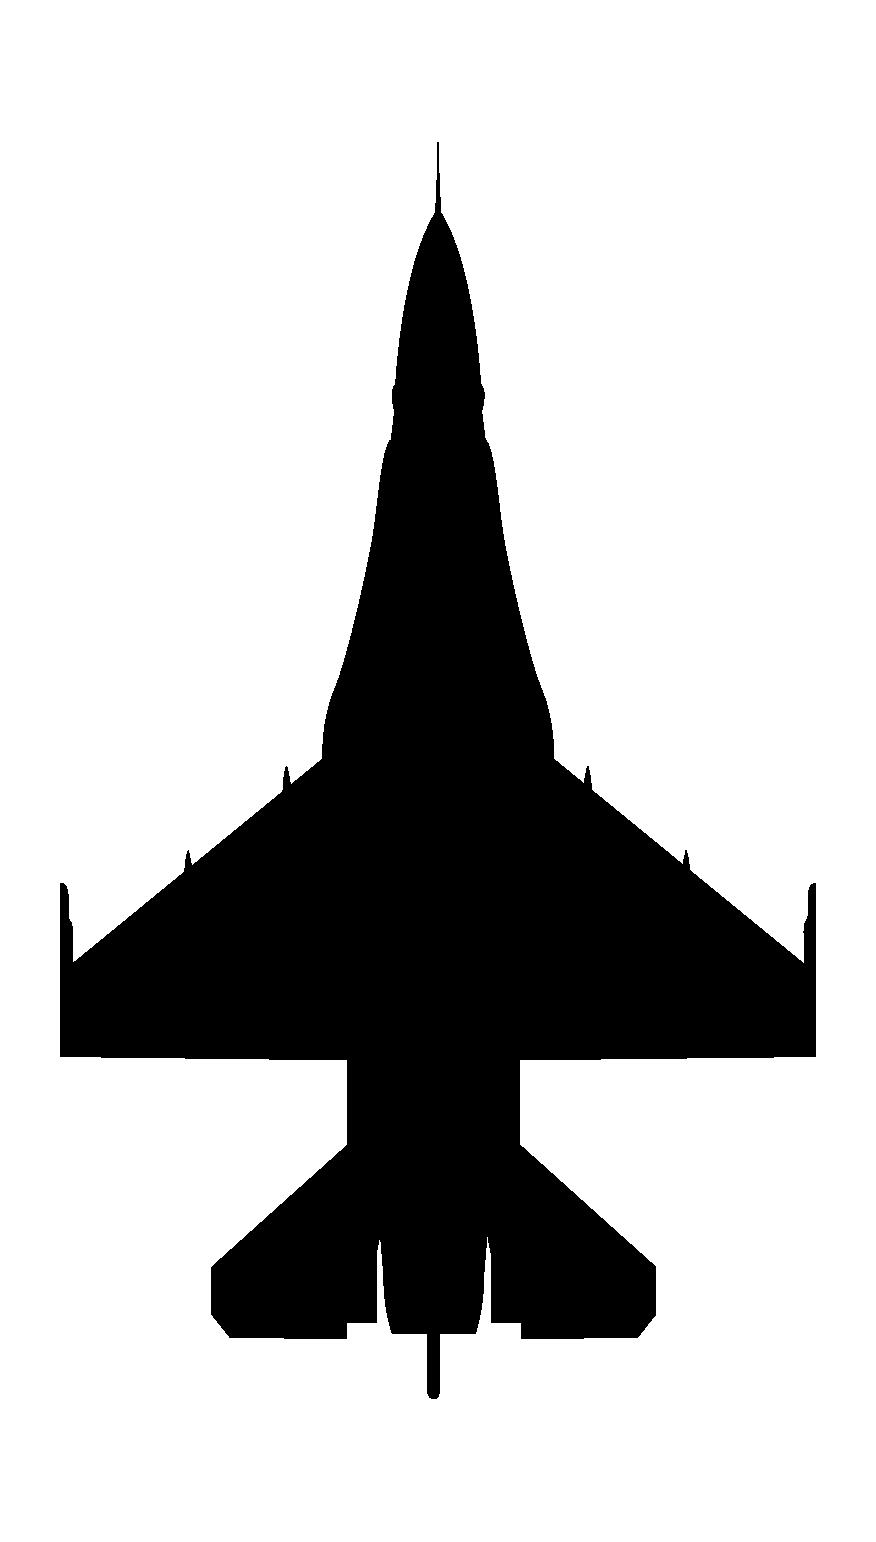
\includegraphics[
                width=7.5mm,
            ]{diagrams/aircraft/silhouette_f16_top.pdf}
        };

        \node[yshift=-2mm] (3fig) at (3) {
            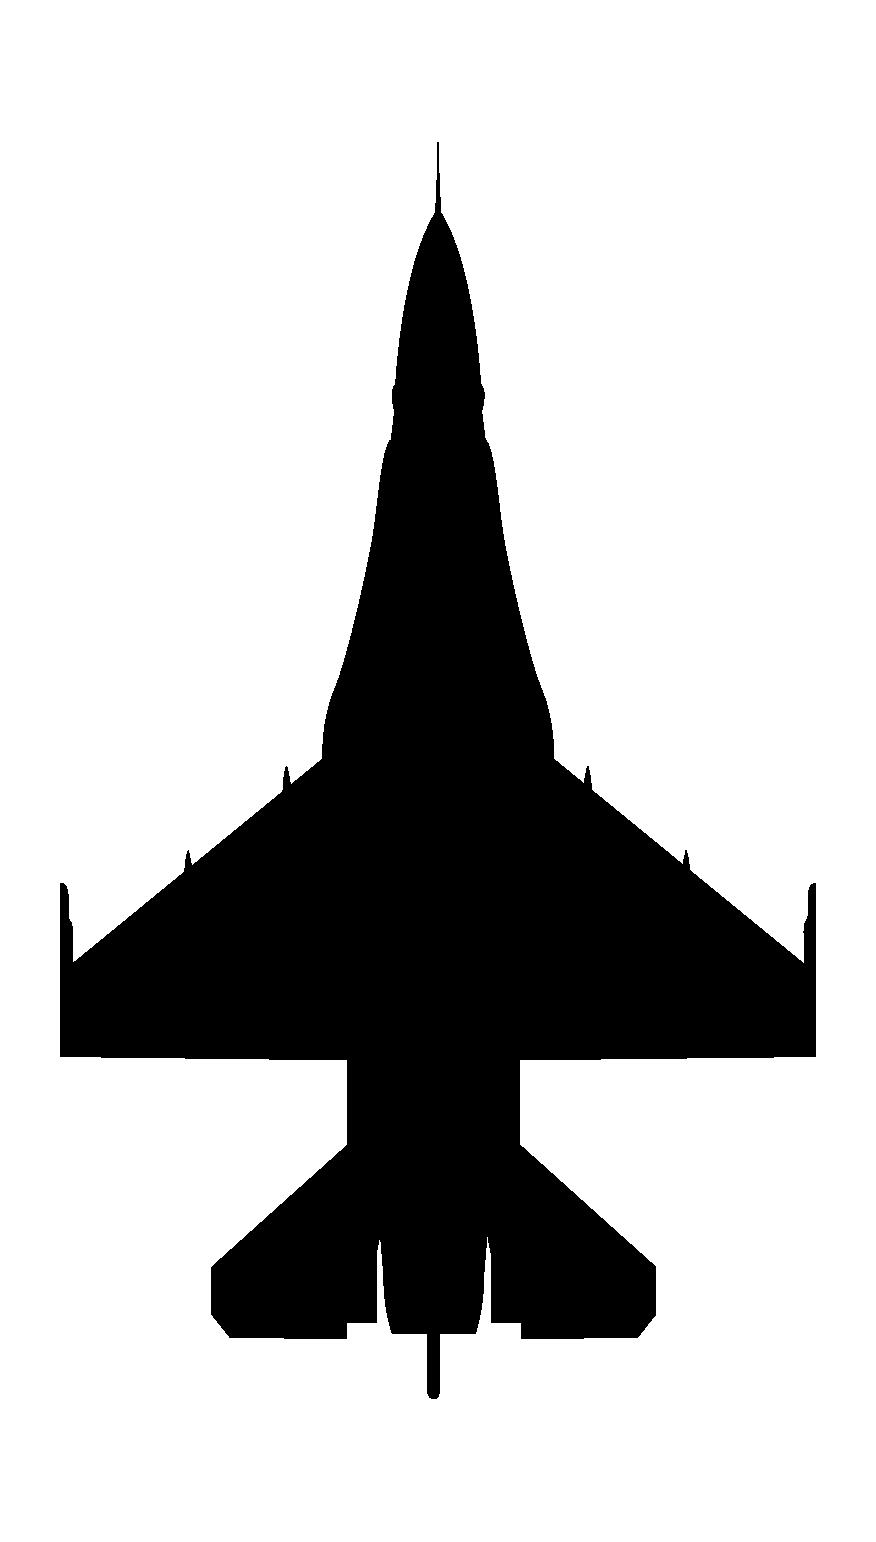
\includegraphics[
                width=7.5mm,
            ]{diagrams/aircraft/silhouette_f16_top.pdf}
        };
        
        \node[yshift=-2mm] (4fig) at (4) {
            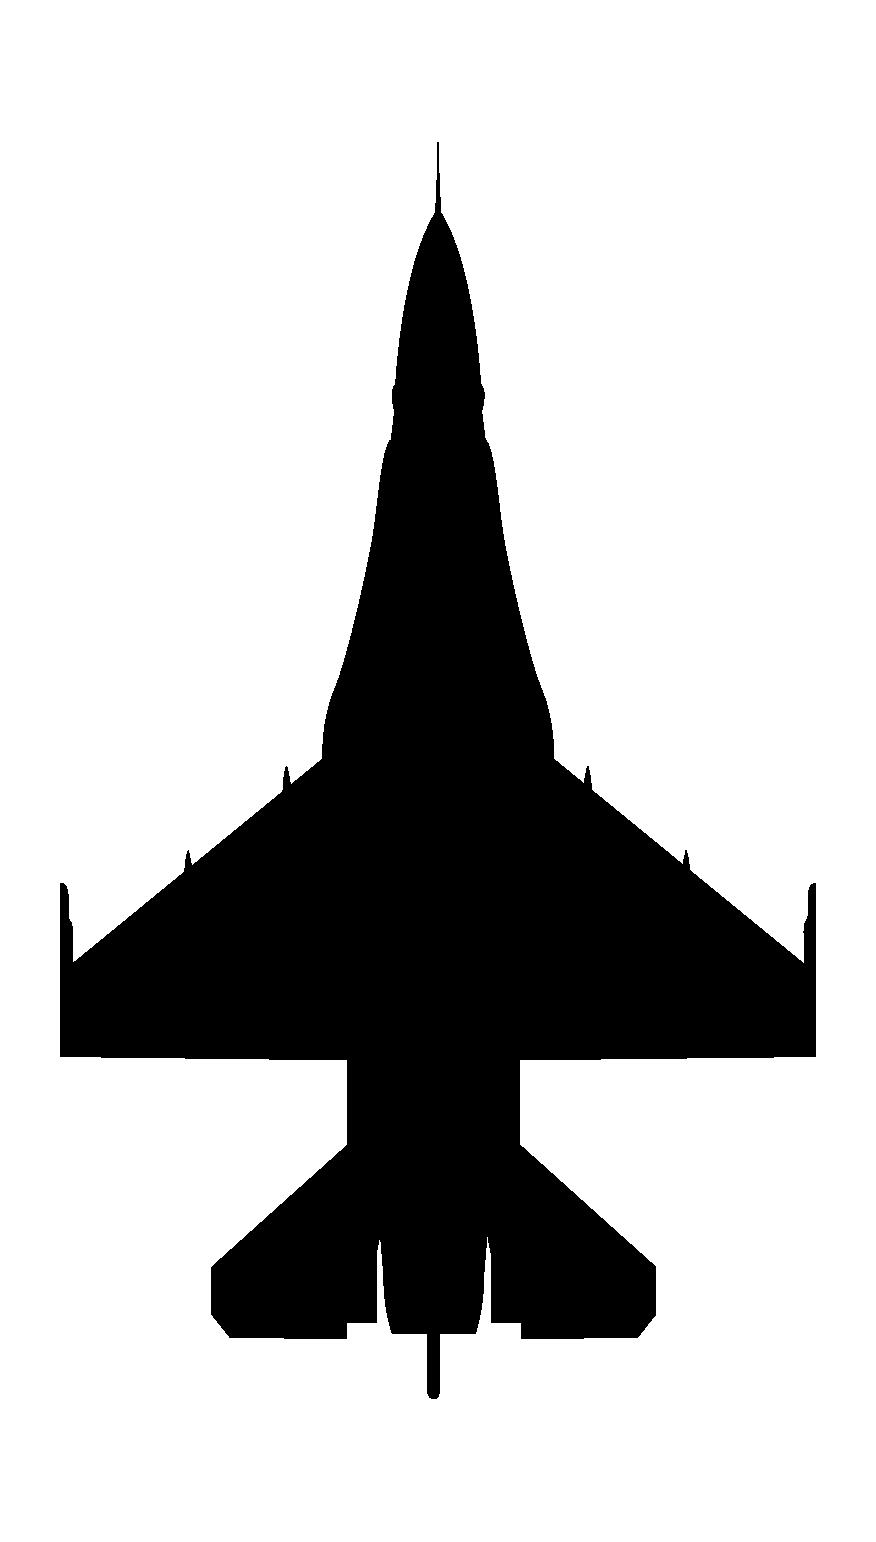
\includegraphics[
                width=7.5mm,
            ]{diagrams/aircraft/silhouette_f16_top.pdf}
        };

        \node[anchor=north, font=\footnotesize] (1label) at (1fig.south) {1};
        \node[anchor=north, font=\footnotesize] (2label) at (2fig.south) {2};
        \node[anchor=north, font=\footnotesize] (3label) at (3fig.south) {3};
        \node[anchor=north, font=\footnotesize] (4label) at (4fig.south) {4};

    \end{tikzpicture}
    \caption{Four-ship offset box formation}
    \label{fig:supp_fig:form:boxoffset}
\end{figure}

\begin{figure}[htbp]
    \centering
    \begin{minipage}[b]{0.5\textwidth}
        \centering
        \begin{tikzpicture}[figstyle]
            
            \coordinate (1) at (0,0);
            \coordinate (2) at ($(1)+(-150:15)$);
            \coordinate (3) at ($(1)+(-30:15)$);
            \coordinate (4) at ($(3)+(-30:15)$);

            \node[yshift=-2mm] (1fig) at (1) {
                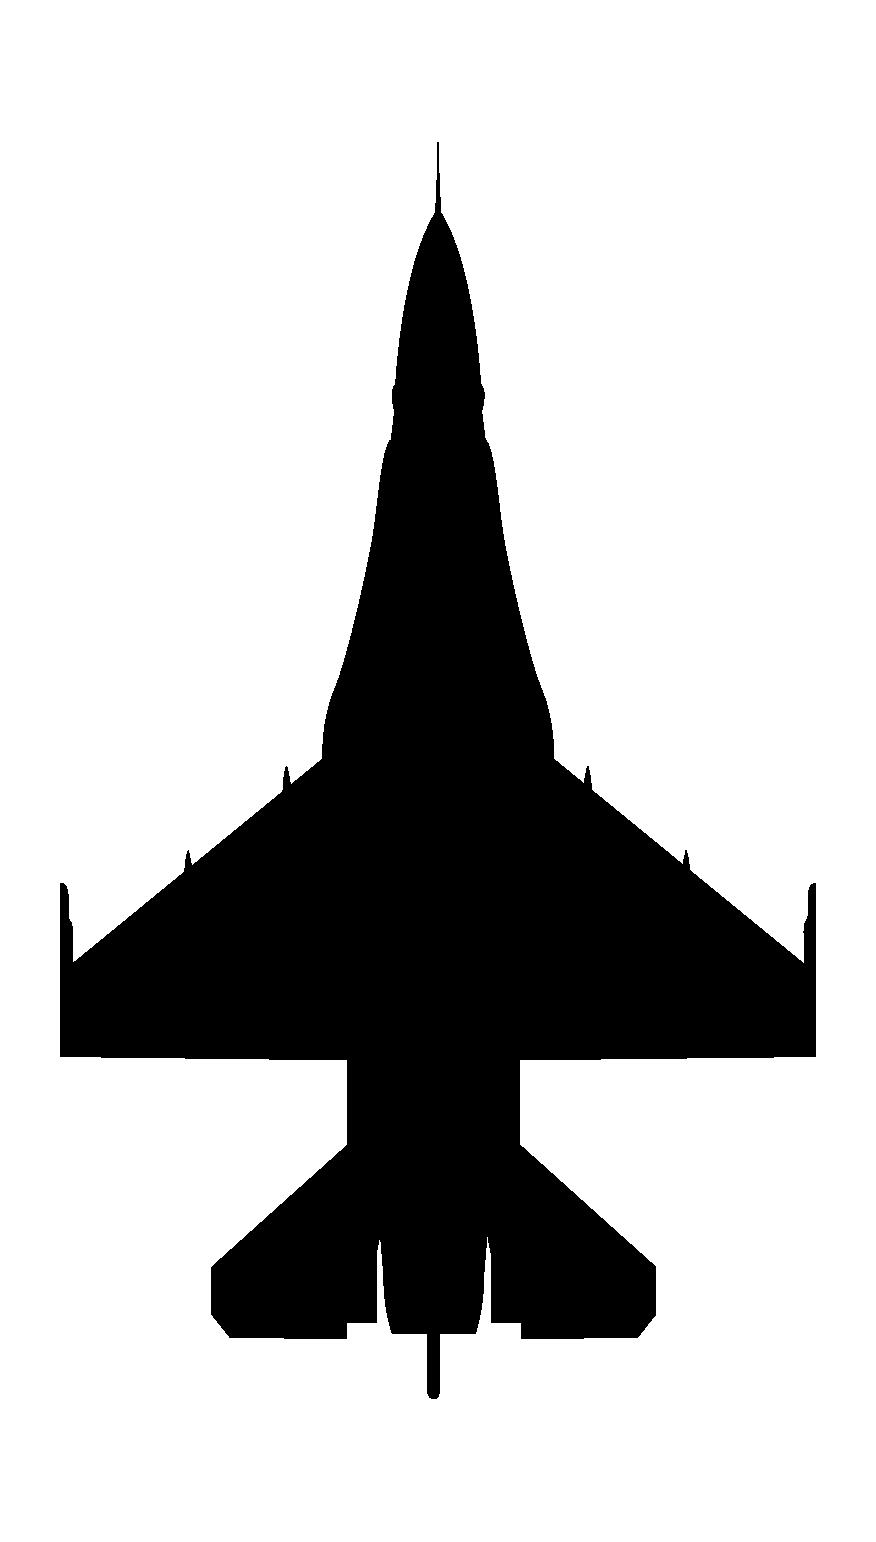
\includegraphics[
                    width=7.5mm,
                ]{diagrams/aircraft/silhouette_f16_top.pdf}
            };
            
            \node[yshift=-2mm] (2fig) at (2) {
                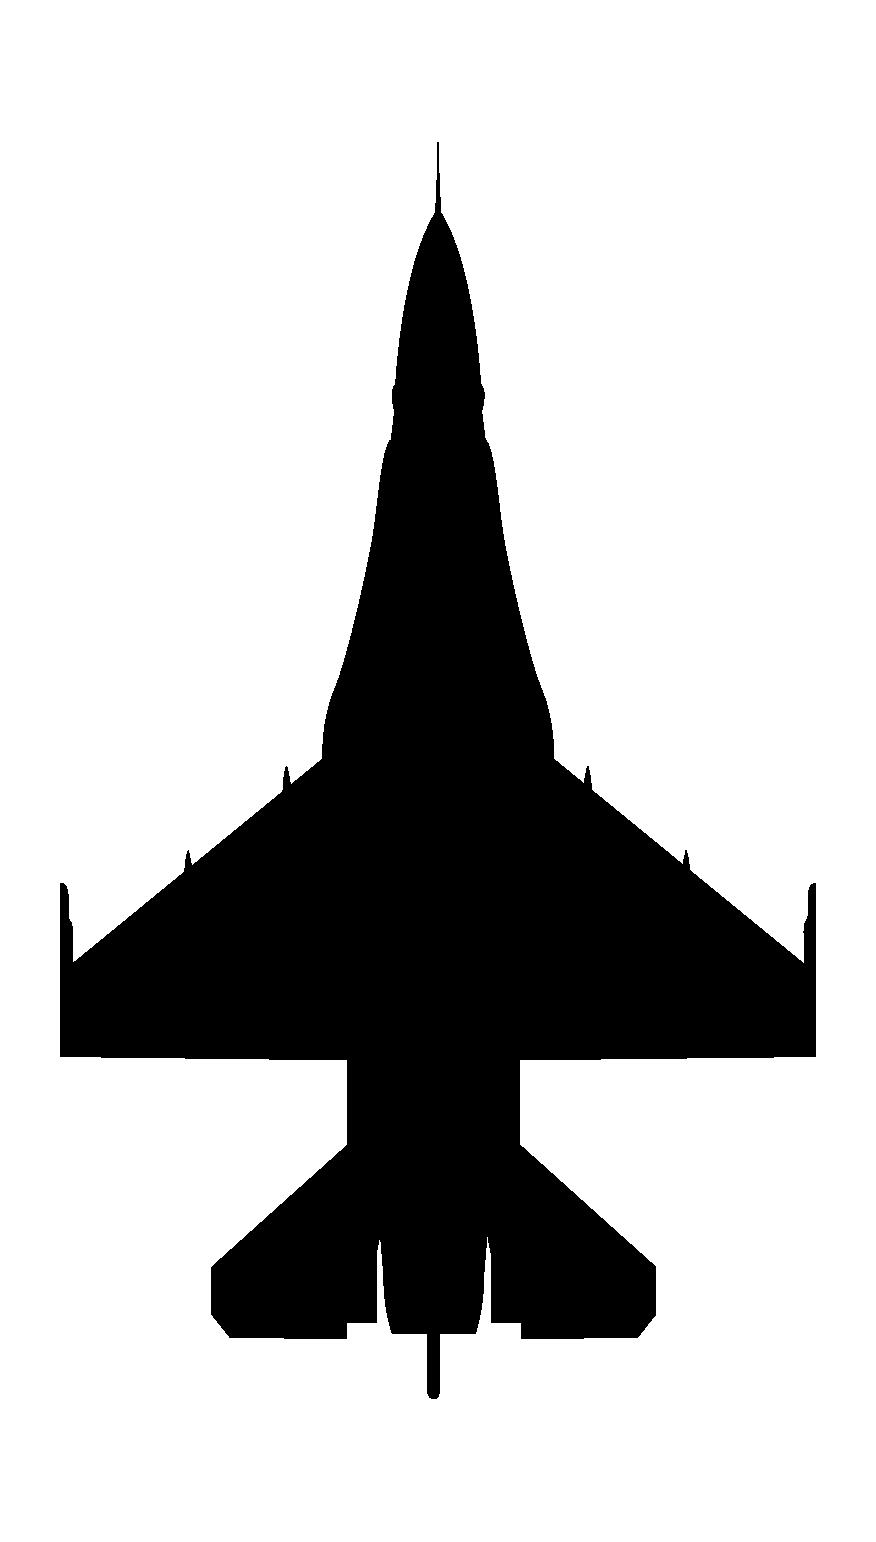
\includegraphics[
                    width=7.5mm,
                ]{diagrams/aircraft/silhouette_f16_top.pdf}
            };

            \node[yshift=-2mm] (3fig) at (3) {
                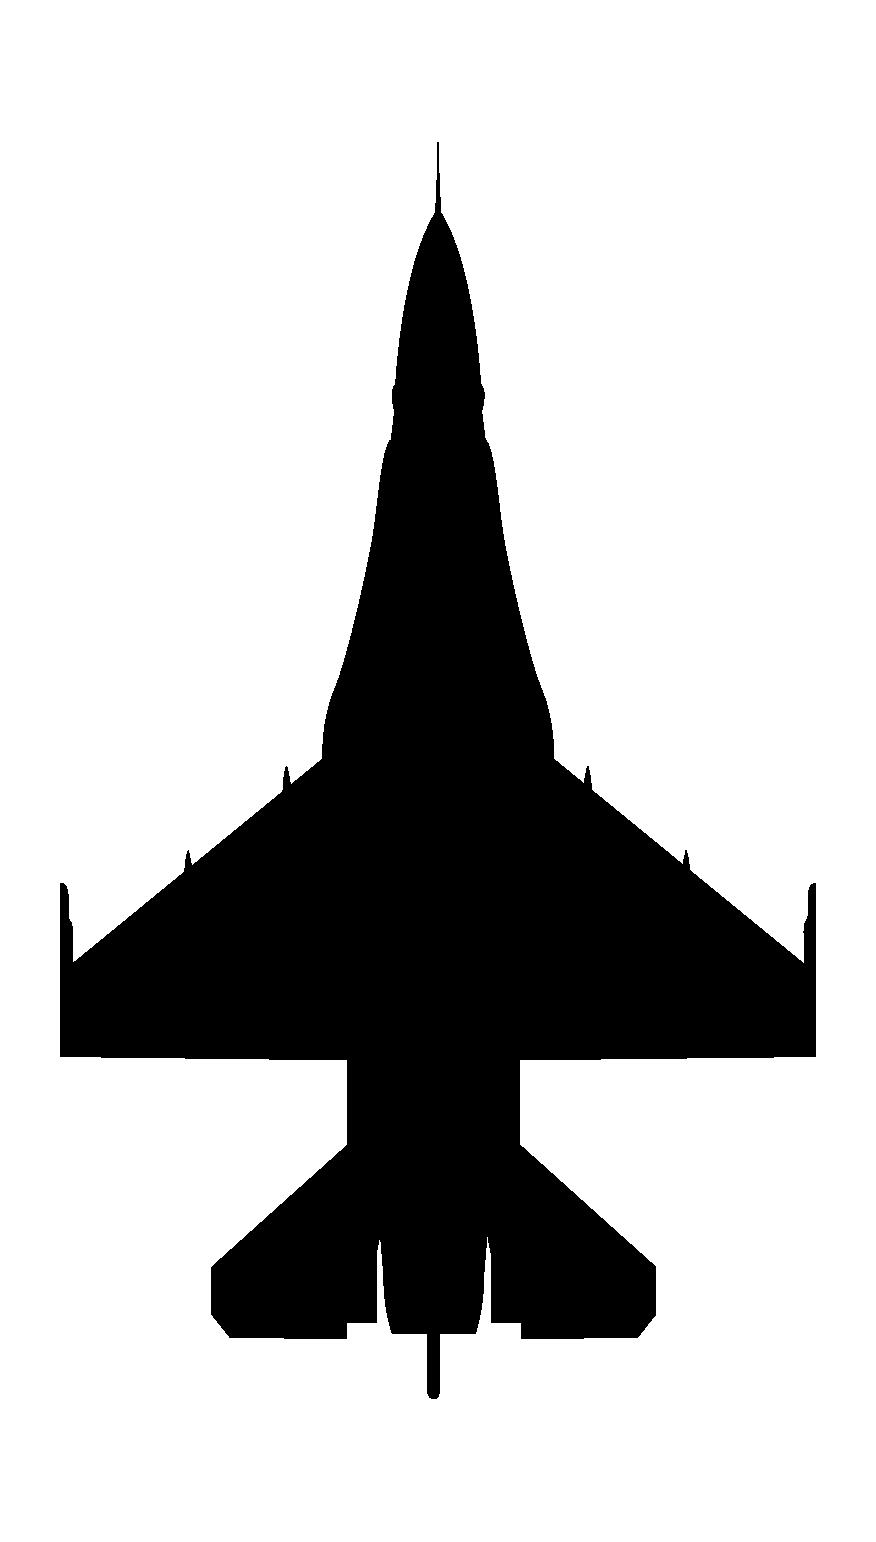
\includegraphics[
                    width=7.5mm,
                ]{diagrams/aircraft/silhouette_f16_top.pdf}
            };
            
            \node[yshift=-2mm] (4fig) at (4) {
                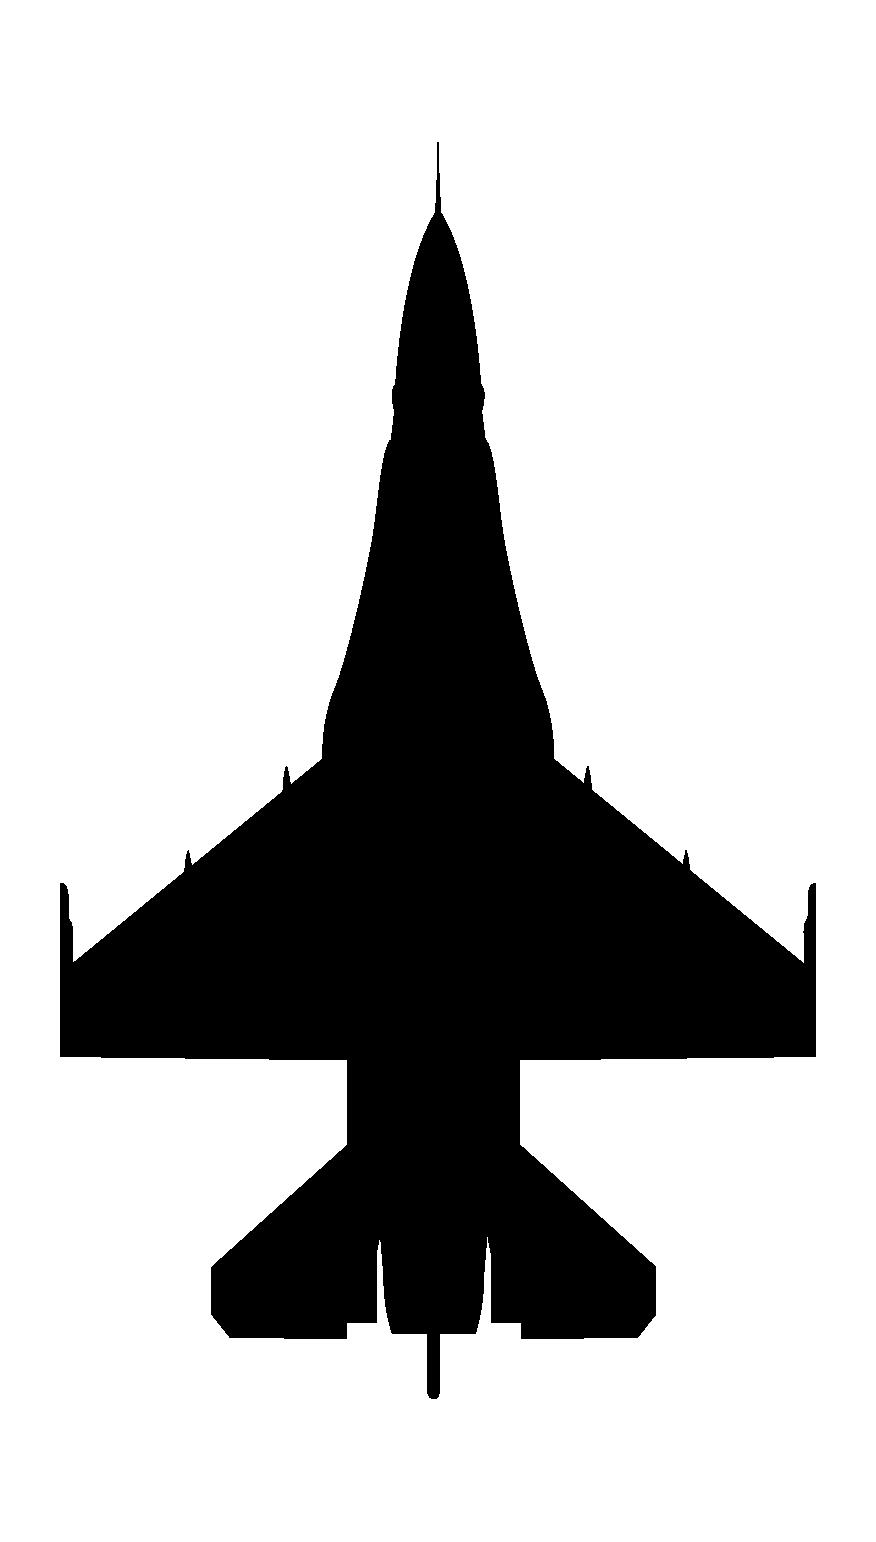
\includegraphics[
                    width=7.5mm,
                ]{diagrams/aircraft/silhouette_f16_top.pdf}
            };

            \node[anchor=north, font=\footnotesize] (1label) at (1fig.south) {1};
            \node[anchor=north, font=\footnotesize] (2label) at (2fig.south) {2};
            \node[anchor=north, font=\footnotesize] (3label) at (3fig.south) {3};
            \node[anchor=north, font=\footnotesize] (4label) at (4fig.south) {4};

        \end{tikzpicture}
        \caption{Fingertip formation}
        \label{fig:supp_fig:form:fingertip}
    \end{minipage}%
    \begin{minipage}[b]{0.5\textwidth}
        \centering
        \begin{tikzpicture}[figstyle]
            
            \coordinate (1) at (0,0);
            \coordinate (2) at ($(1)+(-150:20)$);
            \coordinate (3) at ($(1)+(-30:20)$);
            \coordinate (4) at ($(3)+(-150:20)$);

            \node[yshift=-2mm] (1fig) at (1) {
                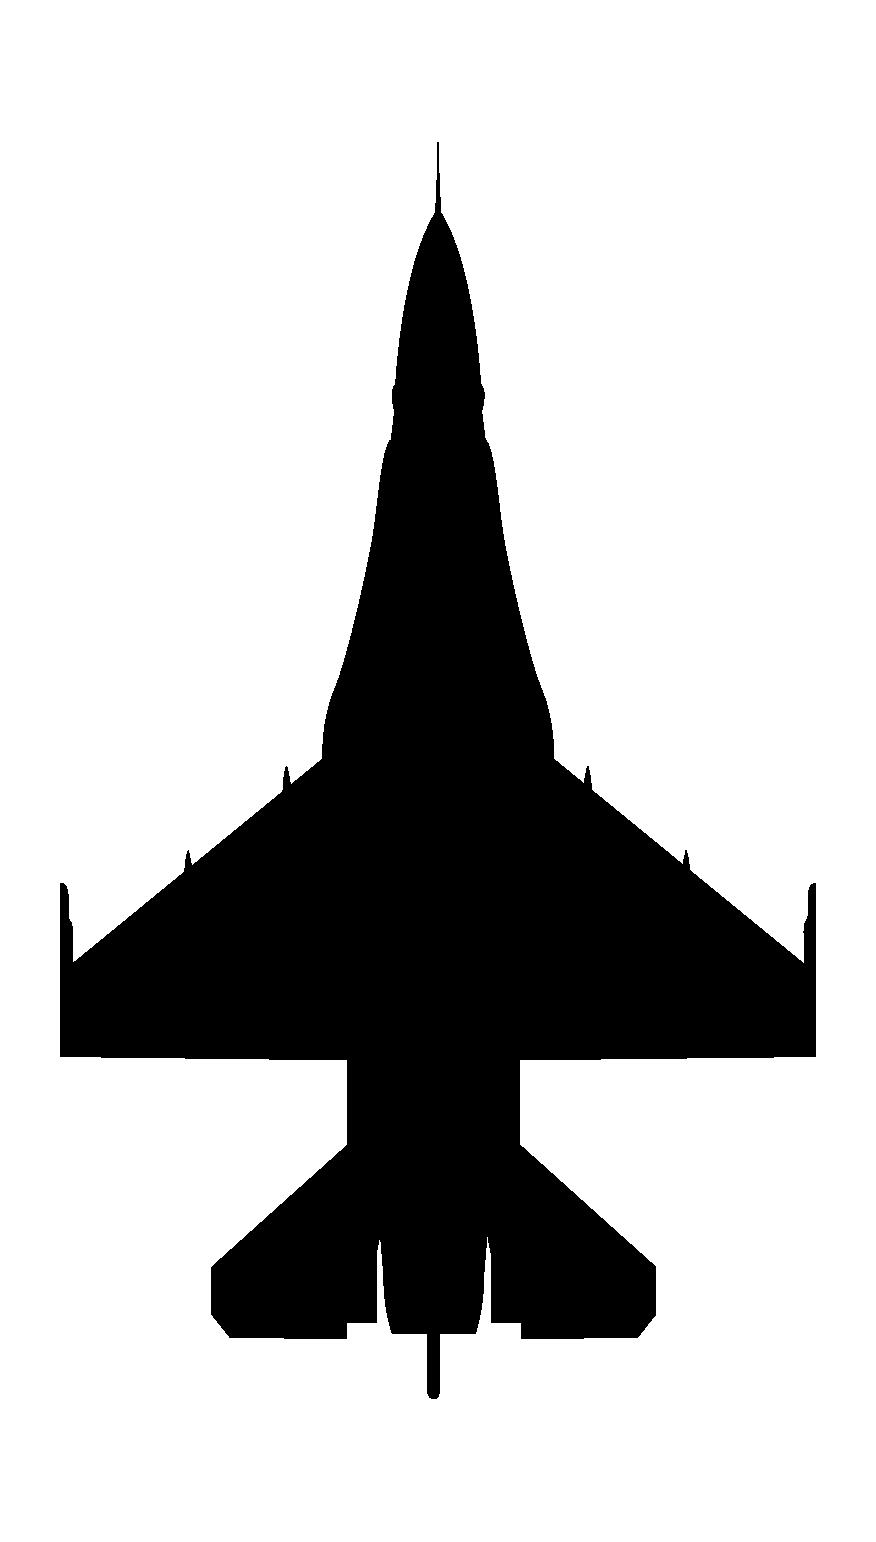
\includegraphics[
                    width=7.5mm,
                ]{diagrams/aircraft/silhouette_f16_top.pdf}
            };
            
            \node[yshift=-2mm] (2fig) at (2) {
                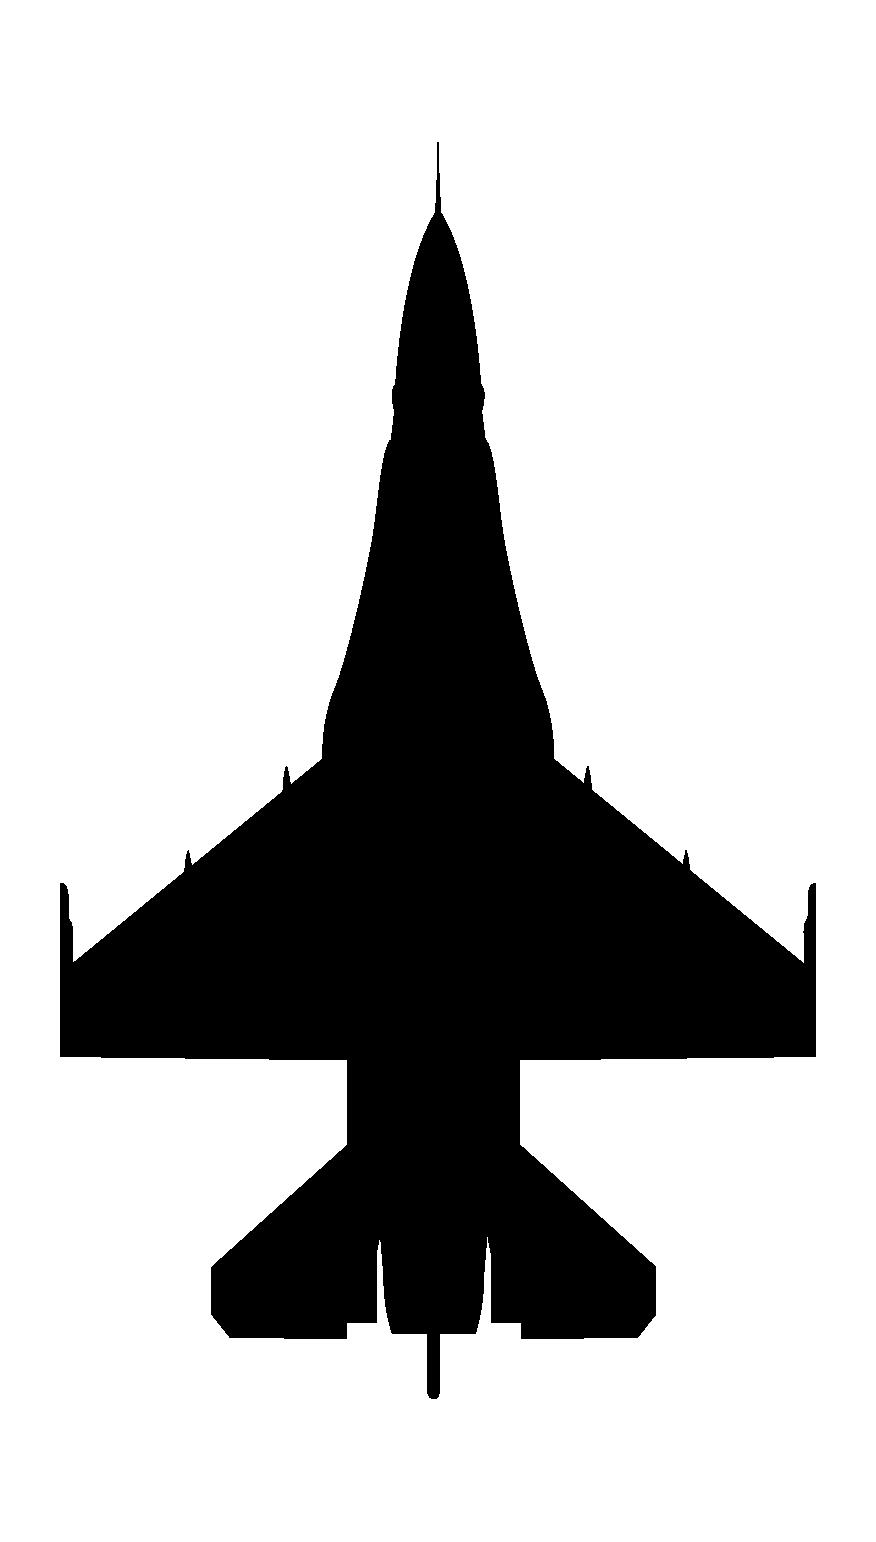
\includegraphics[
                    width=7.5mm,
                ]{diagrams/aircraft/silhouette_f16_top.pdf}
            };

            \node[yshift=-2mm] (3fig) at (3) {
                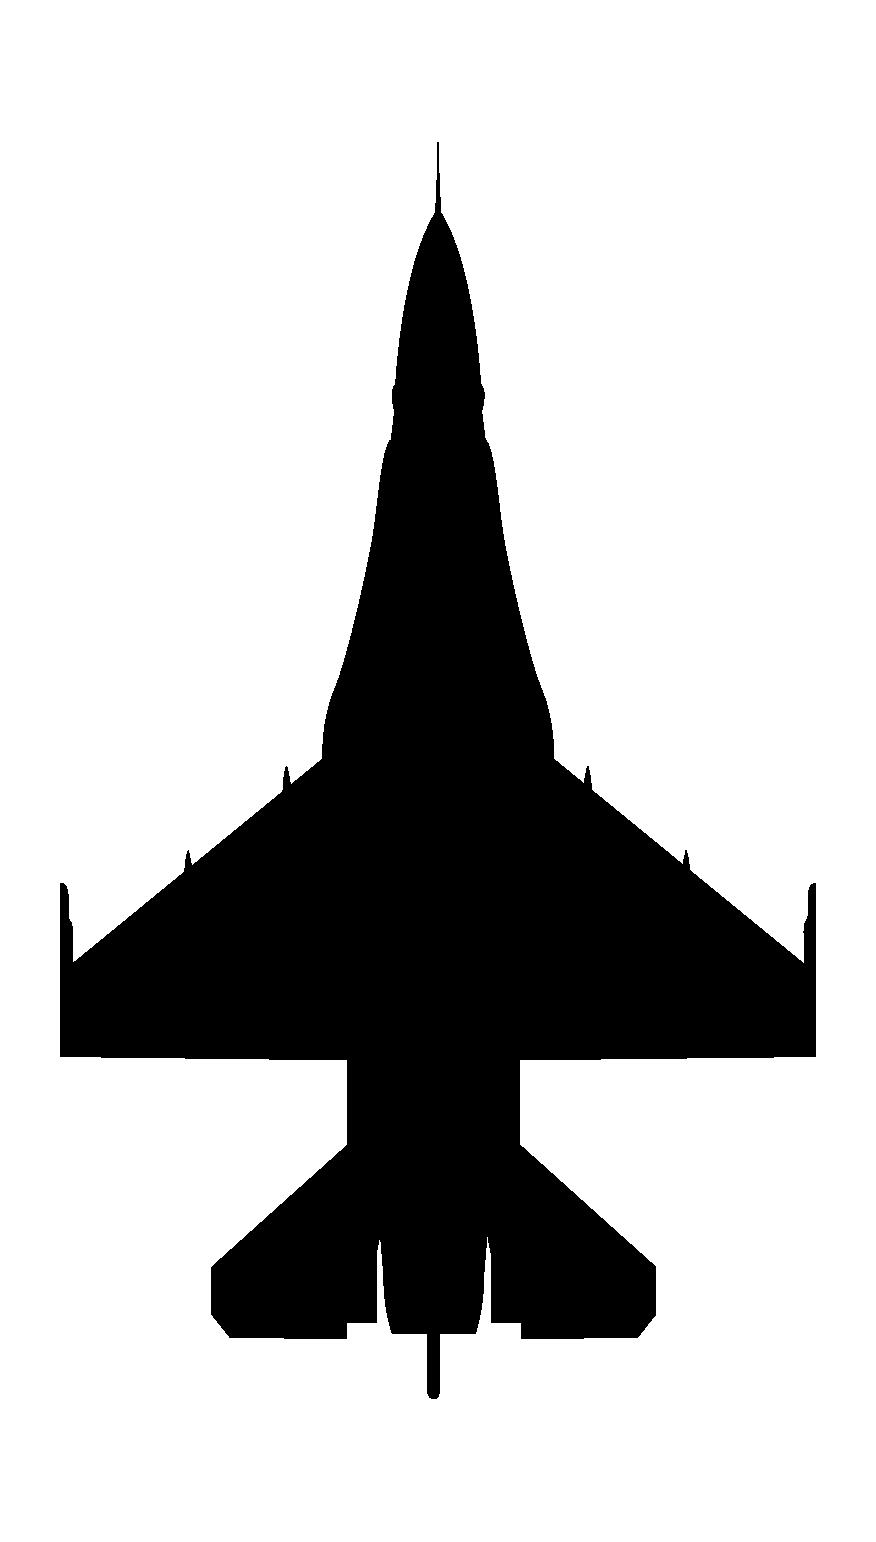
\includegraphics[
                    width=7.5mm,
                ]{diagrams/aircraft/silhouette_f16_top.pdf}
            };
            
            \node[yshift=-2mm] (4fig) at (4) {
                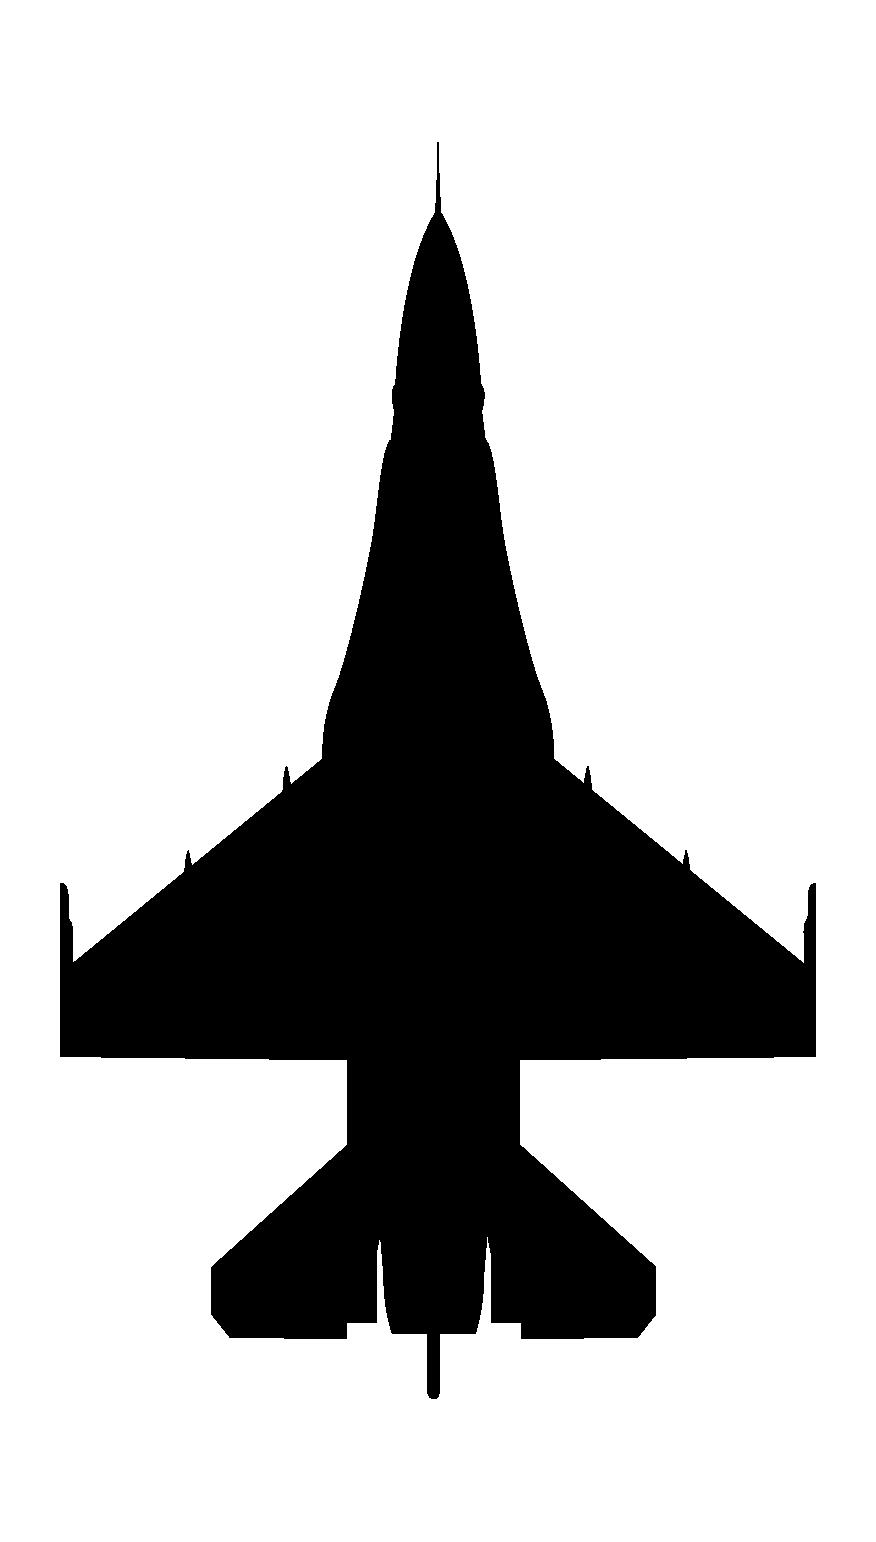
\includegraphics[
                    width=7.5mm,
                ]{diagrams/aircraft/silhouette_f16_top.pdf}
            };

            \node[anchor=north, font=\footnotesize] (1label) at (1fig.south) {1};
            \node[anchor=north, font=\footnotesize] (2label) at (2fig.south) {2};
            \node[anchor=north, font=\footnotesize] (3label) at (3fig.south) {3};
            \node[anchor=north, font=\footnotesize] (4label) at (4fig.south) {4};

        \end{tikzpicture}
        \caption{Diamond formation}
        \label{fig:supp_fig:form:diamond}
    \end{minipage}
\end{figure}

\begin{figure}[htbp]
    \centering
    \begin{minipage}[b]{0.5\textwidth}
        \centering
        \begin{tikzpicture}[figstyle]
            
            \coordinate (1) at (0,0);
            \coordinate (2) at ($(1)+(-90:15)$);
            \coordinate (3) at ($(2)+(-90:15)$);
            \coordinate (4) at ($(3)+(-90:15)$);

            \node[yshift=-2mm] (1fig) at (1) {
                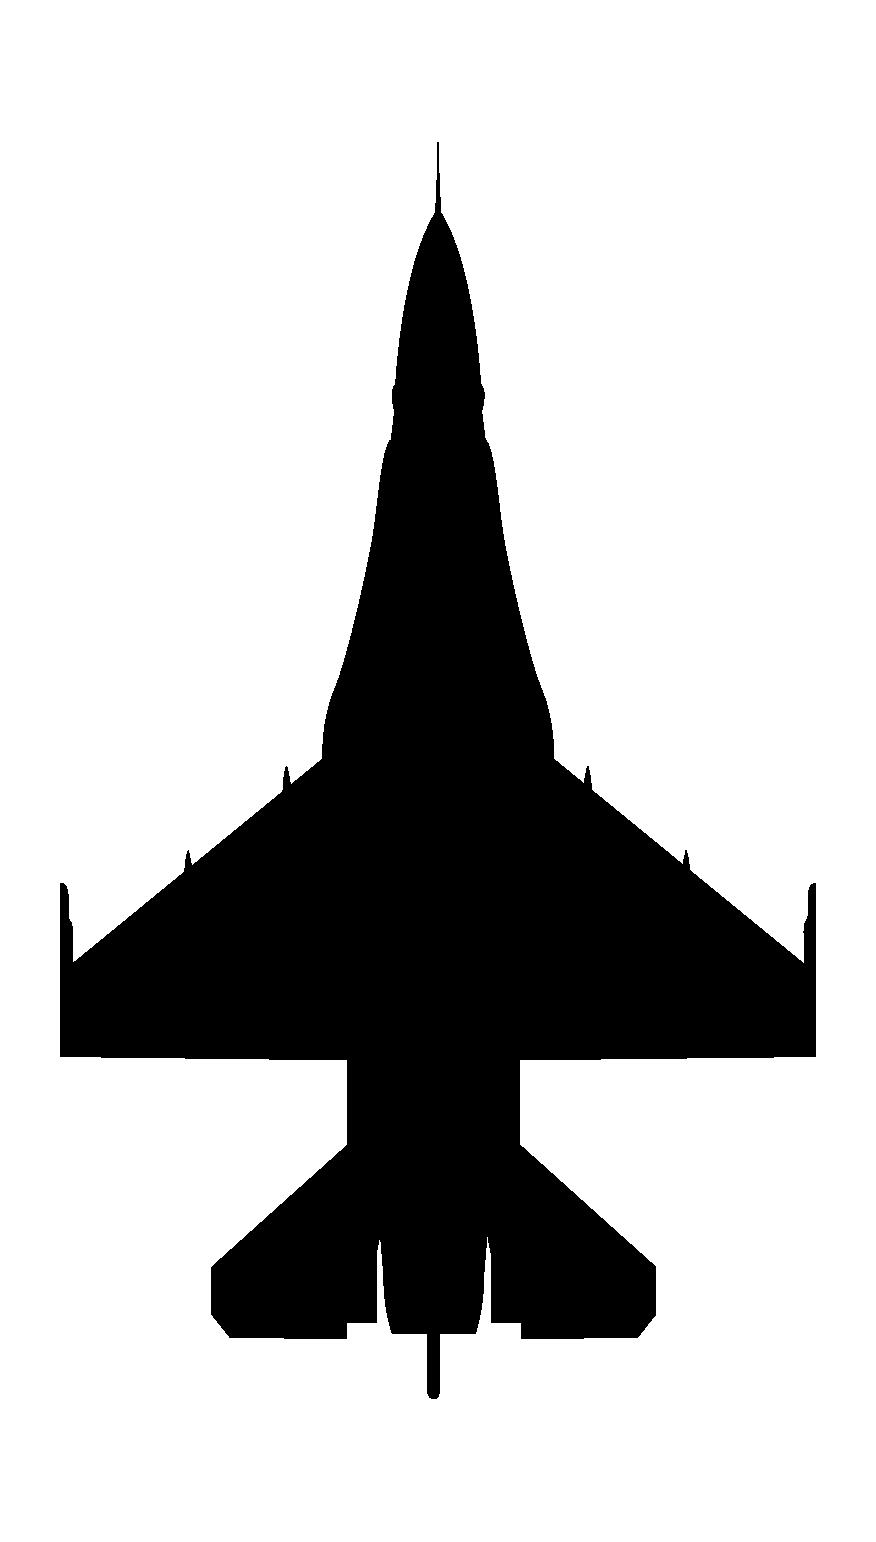
\includegraphics[
                    width=7.5mm,
                ]{diagrams/aircraft/silhouette_f16_top.pdf}
            };
            
            \node[yshift=-2mm] (2fig) at (2) {
                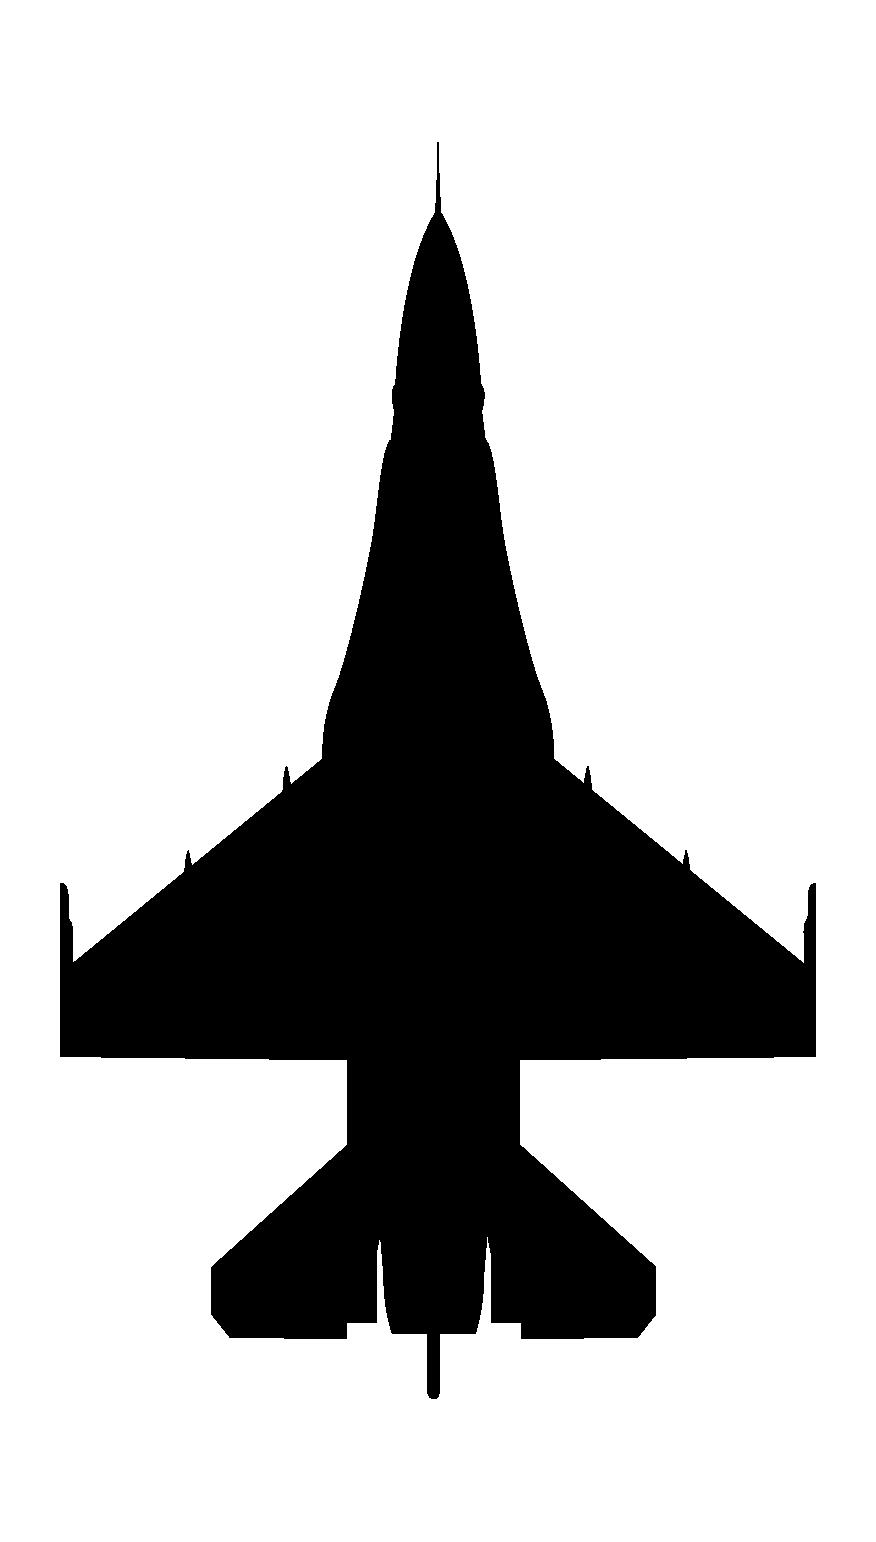
\includegraphics[
                    width=7.5mm,
                ]{diagrams/aircraft/silhouette_f16_top.pdf}
            };

            \node[yshift=-2mm] (3fig) at (3) {
                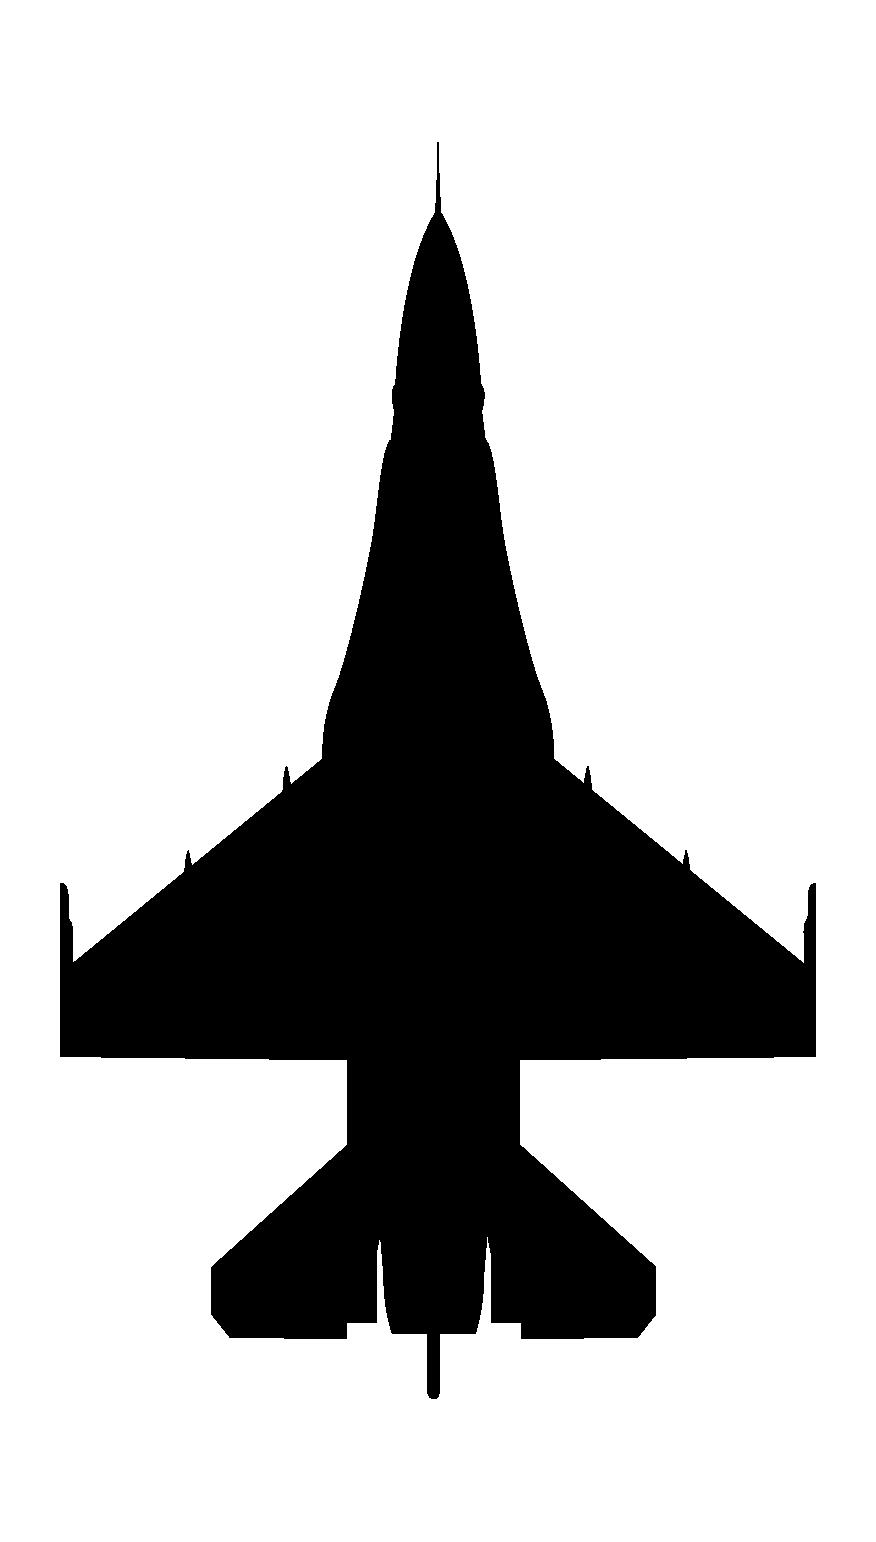
\includegraphics[
                    width=7.5mm,
                ]{diagrams/aircraft/silhouette_f16_top.pdf}
            };
            
            \node[yshift=-2mm] (4fig) at (4) {
                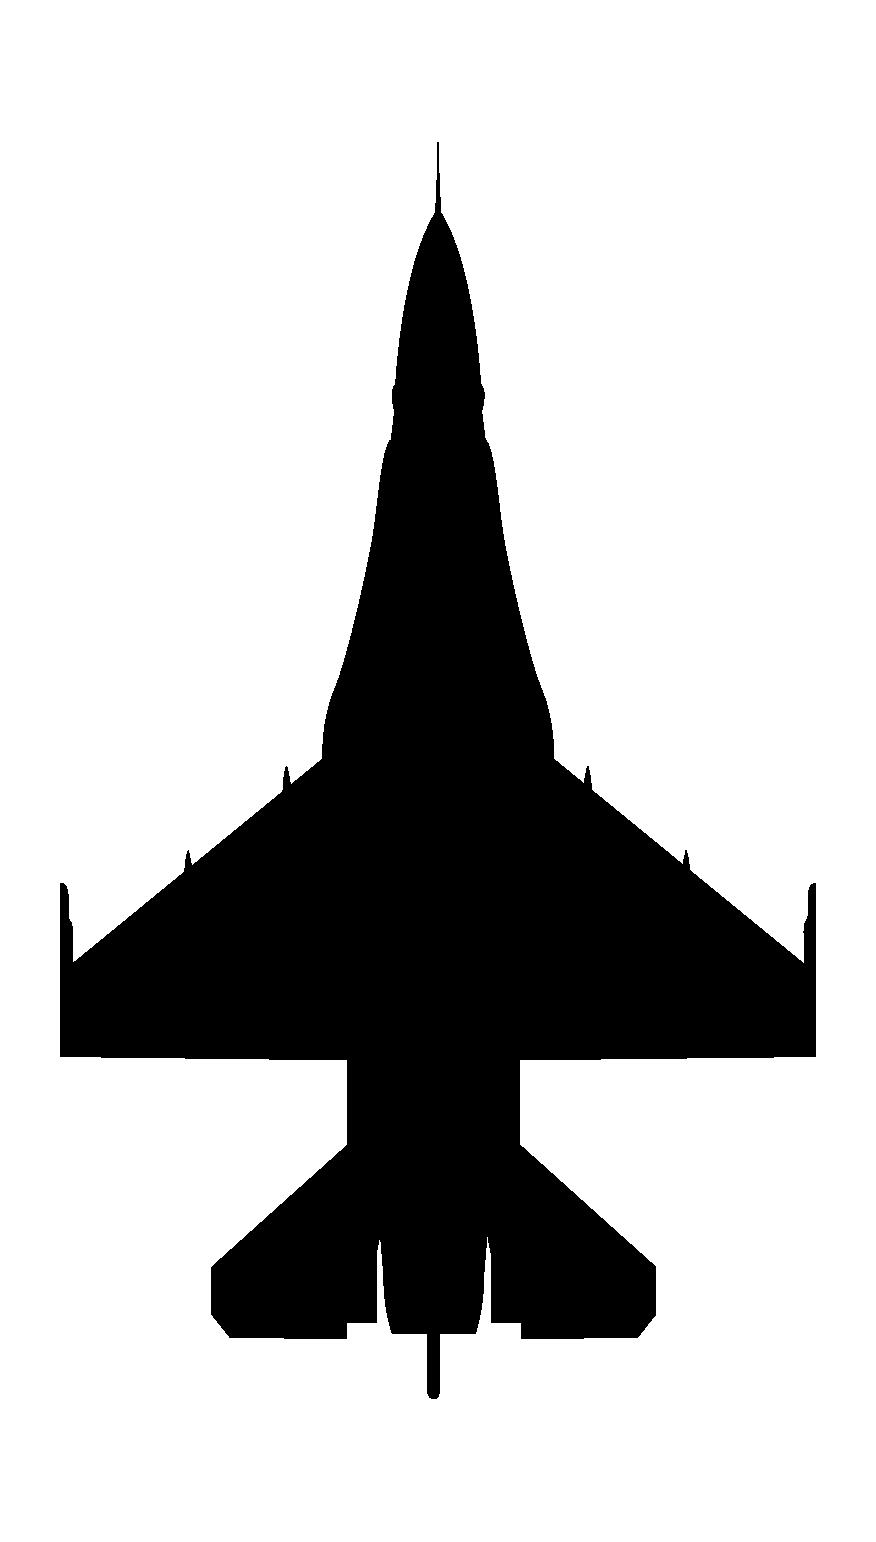
\includegraphics[
                    width=7.5mm,
                ]{diagrams/aircraft/silhouette_f16_top.pdf}
            };

            \node[anchor=west, font=\footnotesize] (1label) at (1fig.east) {1};
            \node[anchor=west, font=\footnotesize] (2label) at (2fig.east) {2};
            \node[anchor=west, font=\footnotesize] (3label) at (3fig.east) {3};
            \node[anchor=west, font=\footnotesize] (4label) at (4fig.east) {4};

        \end{tikzpicture}
        \caption{Trail formation}
        \label{fig:supp_fig:form:trail}
    \end{minipage}%
    \begin{minipage}[b]{0.5\textwidth}
        \centering
        \begin{tikzpicture}[figstyle]
            
            \coordinate (1) at (0,0);
            \coordinate (2) at ($(1)+(0:15)$);
            \coordinate (3) at ($(2)+(0:15)$);
            \coordinate (4) at ($(3)+(0:15)$);

            \node[yshift=-2mm] (1fig) at (1) {
                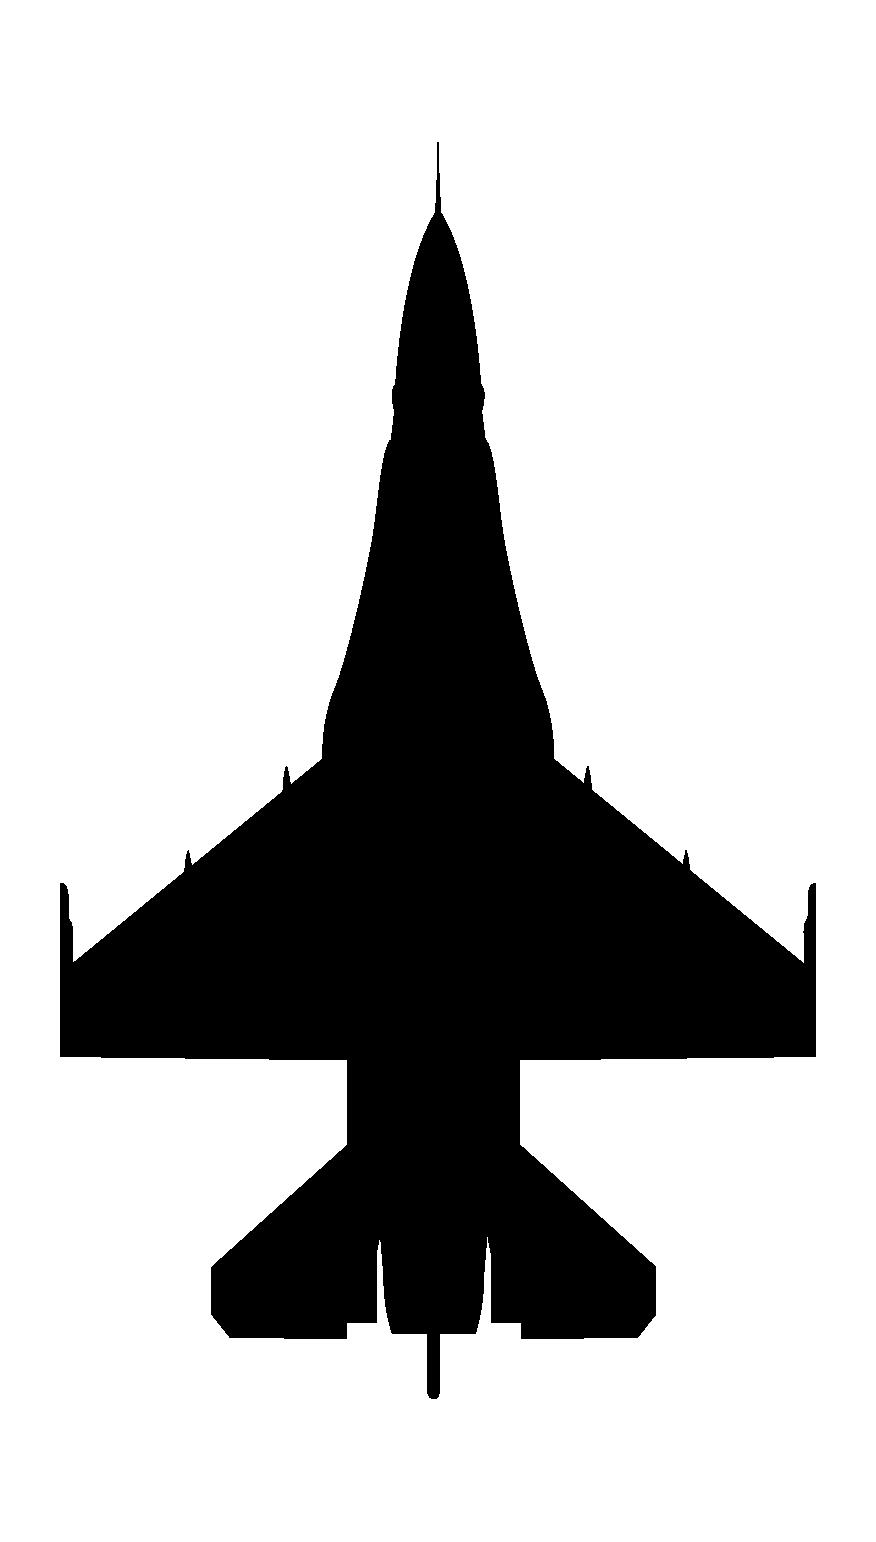
\includegraphics[
                    width=7.5mm,
                ]{diagrams/aircraft/silhouette_f16_top.pdf}
            };
            
            \node[yshift=-2mm] (2fig) at (2) {
                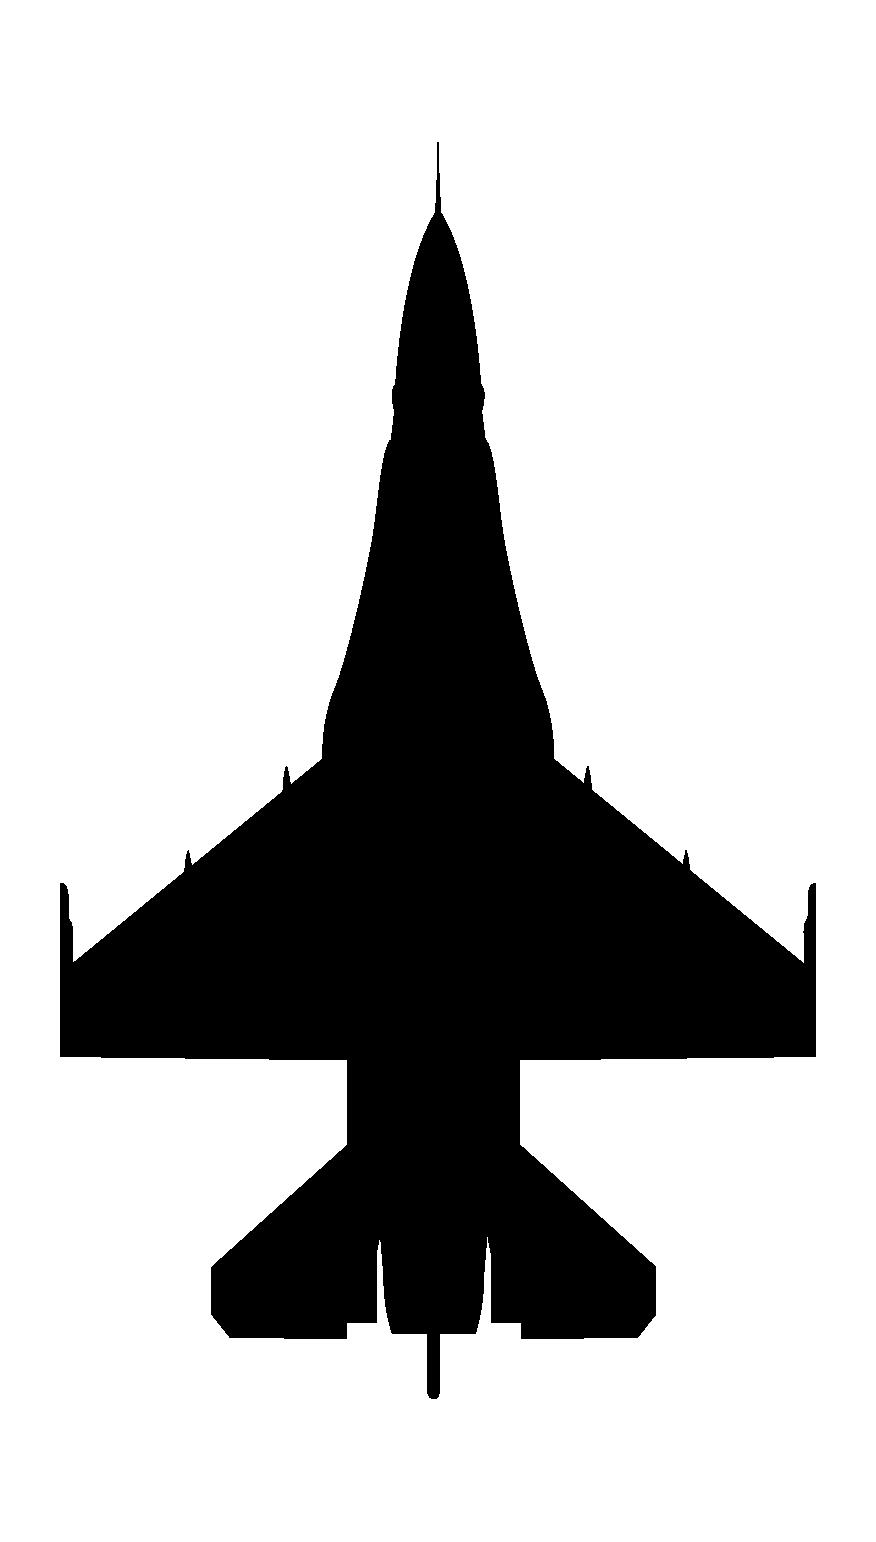
\includegraphics[
                    width=7.5mm,
                ]{diagrams/aircraft/silhouette_f16_top.pdf}
            };

            \node[yshift=-2mm] (3fig) at (3) {
                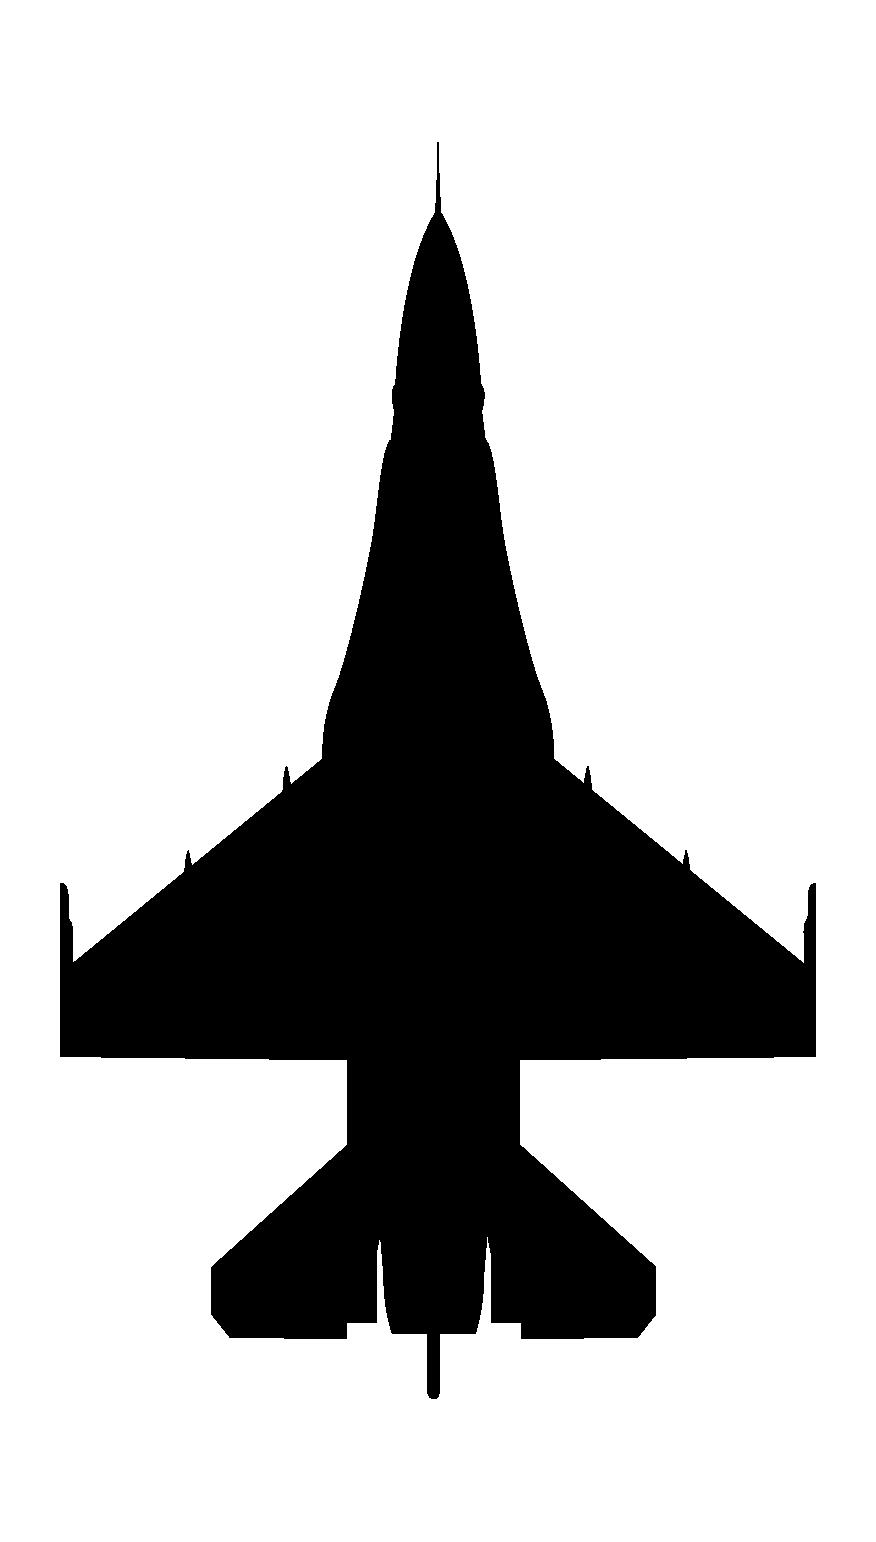
\includegraphics[
                    width=7.5mm,
                ]{diagrams/aircraft/silhouette_f16_top.pdf}
            };
            
            \node[yshift=-2mm] (4fig) at (4) {
                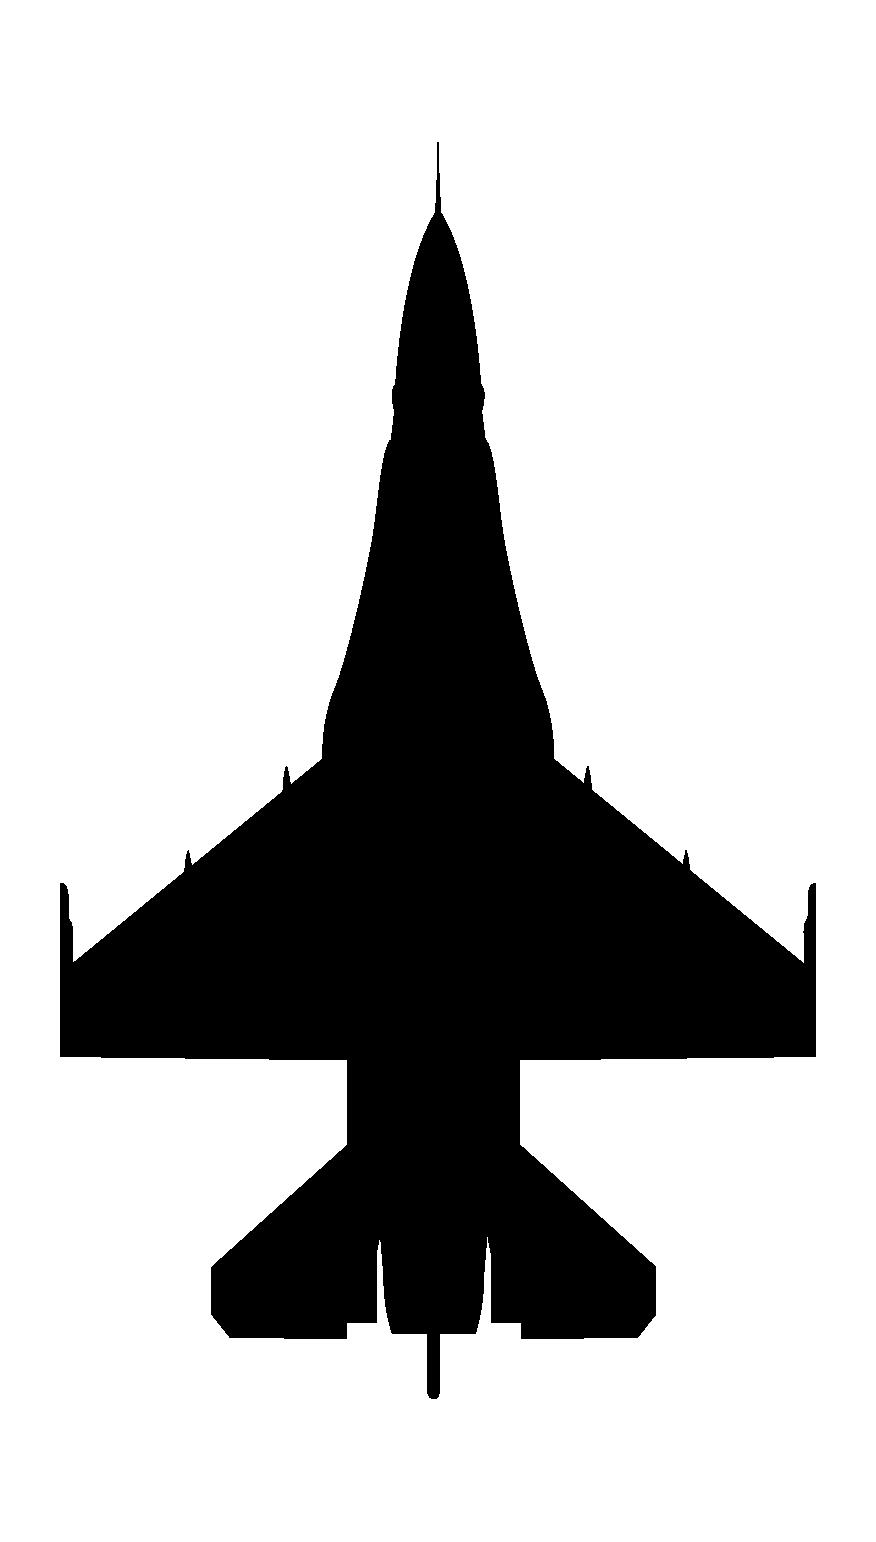
\includegraphics[
                    width=7.5mm,
                ]{diagrams/aircraft/silhouette_f16_top.pdf}
            };

            \node[anchor=north, font=\footnotesize] (1label) at (1fig.south) {1};
            \node[anchor=north, font=\footnotesize] (2label) at (2fig.south) {2};
            \node[anchor=north, font=\footnotesize] (3label) at (3fig.south) {3};
            \node[anchor=north, font=\footnotesize] (4label) at (4fig.south) {4};

        \end{tikzpicture}
        \caption{Spread formation}
        \label{fig:supp_fig:form:spread}
    \end{minipage}
\end{figure}

\clearpage